\documentclass[a4paper]{article}
\usepackage[T1]{fontenc}			% \chapter package
\usepackage[italian]{babel}
\usepackage[italian]{isodate}  		% date format
\usepackage{graphicx}				% manage images
\usepackage{amsfonts}
\usepackage{booktabs}				% high quality tables
\usepackage{amsmath}				% math package
\usepackage{amssymb}				% another math package (e.g. \nexists)
\usepackage{bm}                     % bold math symbols
\usepackage{mathtools}				% emphasize equations
\usepackage{stmaryrd} 				% '\llbracket' and '\rrbracket'
\usepackage{amsthm}					% better theorems
\usepackage{enumitem}				% manage list
\usepackage{pifont}					% nice itemize
\usepackage{cancel}					% cancel math equations
\usepackage{caption}				% custom caption
\usepackage[]{mdframed}				% box text
\usepackage{multirow}				% more lines in a table
\usepackage{textcomp, gensymb}		% degree symbol
\usepackage[x11names]{xcolor}		% RGB color
\usepackage[many]{tcolorbox}				% colorful box
\usepackage{multicol}				% more rows in a table (used for the lists)
\usepackage{listings}
\usepackage{url}
\usepackage{qrcode}
\usepackage{fontawesome5}
\usepackage{ragged2e}
\usepackage{cite}                   % references
\usepackage{imakeidx}               % index
\makeindex[program=makeindex, columns=1,
           title=Index, 
           intoc,
           options={-s index-style.ist}]
\usepackage{fancyhdr}

%\pdfcompresslevel=0
%\pdfobjcompresslevel=0

\definecolor{codegreen}{rgb}{0,0.6,0}
\definecolor{codegray}{rgb}{0.5,0.5,0.5}
\definecolor{codepurple}{rgb}{0.58,0,0.82}
\definecolor{backcolour}{rgb}{0.95,0.95,0.92}
\lstdefinestyle{mystyle}{
    backgroundcolor=\color{backcolour},   
    commentstyle=\color{codegreen},
    keywordstyle=\color{magenta},
    numberstyle=\tiny\color{codegray},
    stringstyle=\color{codepurple},
    basicstyle=\ttfamily\footnotesize,
    breakatwhitespace=false,         
    breaklines=true,                 
    captionpos=b,                    
    keepspaces=true,                 
    numbers=left,                    
    numbersep=5pt,                  
    showspaces=false,                
    showstringspaces=false,
    showtabs=false,                  
    tabsize=2
}
\lstset{style=mystyle}


% draw a frame around given text
\newcommand{\framedtext}[1]{%
	\par%
	\noindent\fbox{%
		\parbox{\dimexpr\linewidth-2\fboxsep-2\fboxrule}{#1}%
	}%
}


% table of content links
\usepackage{xcolor}
\usepackage[linkcolor=black, citecolor=blue, urlcolor=cyan]{hyperref} % hypertexnames=false
\hypersetup{
	colorlinks=true
}


\newtheorem{theorem}{\textcolor{Red3}{\underline{Theorem}}}
\renewcommand{\qedsymbol}{QED}
\newcommand{\dquotes}[1]{``#1''}
\newcommand{\longline}{\noindent\rule{\textwidth}{0.4pt}}
\newcommand{\circledtext}[1]{\raisebox{.5pt}{\textcircled{\raisebox{-.9pt}{#1}}}}
\newcommand{\definition}[1]{\textcolor{Red3}{\textbf{#1}}\index{#1}}
\newcommand{\example}[1]{\textcolor{Green4}{\textbf{#1}}}
\newcommand{\highspace}{\vspace{1.2em}\noindent}
\newenvironment{rowequmat}[1]{\left(\array{@{}#1@{}}}{\endarray\right)}
\newenvironment{rowequmatbra}[1]{\left[\array{@{}#1@{}}}{\endarray\right]}

\begin{document}
    \newcounter{definition}[section]
    \newcounter{example}[section]
    
    \newtcolorbox[use counter = definition]{definitionbox}[1][]{%
        colback=red!5!white,
        colframe=red!75!black,
        fonttitle=\bfseries,
        title={Definizione \thetcbcounter #1} %
    }
    
    \newtcolorbox[use counter = example]{examplebox}[1][]{%
        breakable,
        enhanced,
        colback=Green4!5!white,
        colframe=Green4!75!black,
        fonttitle=\bfseries,
        title={Esempio \thetcbcounter #1} %
    }

    %%%%%%%%%%%%%%%
    % Notes cover %
    %%%%%%%%%%%%%%%
    \author{260236}
\title{Parallel Computing - Notes - \version}
\date{\printdayoff\today}
\maketitle

    %%%%%%%%%%%
    % Preface %
    %%%%%%%%%%%
	\section*{Preface}

Every theory section in these notes has been taken from the sources:
\begin{itemize}
    \item Course slides.\cite{numerical-linear-algebra-polimi}
\end{itemize}
About:
\begin{itemize}
    \item[\faIcon{github}] \href{https://github.com/PoliMI-HPC-E-notes-projects-AndreVale69/HPC-E-PoliMI-university-notes}{GitHub repository}
    \begin{center}
        \qrcode{https://github.com/PoliMI-HPC-E-notes-projects-AndreVale69/HPC-E-PoliMI-university-notes}
    \end{center}
\end{itemize}
These notes are an unofficial resource and shouldn't replace the course material or any other book on numerical linear algebra. It is not made for commercial purposes. I've made the following notes to help me improve my knowledge and maybe it can be helpful for everyone.

As I have highlighted, a student should choose the teacher's material or a book on the topic. These notes can only be a helpful material.

\highspace

\subsection*{Correlated Projects}

During the Numerical Linear Algebra for HPC course, I was part of a team where we created a project that included two challenges related to the course. See more details in the corresponding repository:
\begin{itemize}
    \item[\faIcon{github}] \href{https://github.com/PoliMI-HPC-E-notes-projects-AndreVale69/NLA-challenges}{GitHub repository}
    \begin{center}
        \qrcode{https://github.com/PoliMI-HPC-E-notes-projects-AndreVale69/NLA-challenges}
    \end{center}
\end{itemize}

    %%%%%%%%%%%%%%%%%%%%%
    % Table of contents %
    %%%%%%%%%%%%%%%%%%%%%
    \tableofcontents
    \newpage

    %%%%%%%%%%%%%%%%%%%
    % Fancy pagestyle %
    %%%%%%%%%%%%%%%%%%%
    \pagestyle{fancy}
    \fancyhead{} % clear all header fields
    \fancyhead[R]{\nouppercase{\leftmark\hfill\rightmark}}

    %%%%%%%%%%%%%%%%%%%%%%%%%
    % Equazioni non lineari %
    %%%%%%%%%%%%%%%%%%%%%%%%%
    \include{sections/equazioni-non-lineari/introduzione-metodo-di-bisezione}
    \subsection{Il metodo di Newton}\label{subsection: il metodo di newton per sistemi lineari}

Il \definition{metodo di Newton} sfrutta la funzione $f$ maggiormente rispetto al metodo di bisezione, usando i suoi valori e la sua derivata.

\highspace
Si ricorda che la retta tangente alla curva $\left(x, f\left(x\right)\right)$ nel punto $x^{(k)}$ è:
\begin{equation*}
    y\left(x\right) = f\left(x^{(k)}\right) + f'\left(x^{(k)}\right)\left(x-x^{(k)}\right)
\end{equation*}
\textbf{Cercando} un $x^{\left(k+1\right)}$ tale che la \textbf{retta tangente in quel punto sia uguale a zero} $y\left(x^{\left(k+1\right)}\right) = 0$, allora si trova:
\begin{equation}\label{eq: metodo di Newton}
    x^{\left(k+1\right)} = x^{\left(k\right)} - \dfrac{f\left(x^{\left(k\right)}\right)}{f'\left(x^{\left(k\right)}\right)} \hspace{2em} k \ge 0
\end{equation}
Purché la derivata prima nel punto $x^{(k)}$ sia diversa da zero, cioè $f'\left(x^{k}\right) \ne 0$.

\highspace
Questa equazione consente di calcolare una successione di valori $x^{(k)}$ a partire da un dato iniziale $x^{(0)}$. In altre parole, il \textbf{metodo di Newton calcola lo zero di $f$ sostituendo localmente a $f$ la sua retta tangente}.

\highspace
A differenza del metodo di bisezione, tale \textbf{metodo converge allo zero in un solo passo quando la funzione $f$ è lineare}, ovvero nella forma $f\left(x\right) = a_{1}x + a_{0}$.

\begin{flushleft}
    \textcolor{Red2}{\faIcon{exclamation-triangle} \textbf{Limitazione}}
\end{flushleft}
La \textbf{convergenza} del metodo di Newton \underline{non} è garantita \textbf{per ogni scelta} di $x^{(0)}$, ma \textbf{soltanto} per valori di $x^{(0)}$ \textbf{sufficientemente vicini} ad $\alpha$, ovvero \textbf{appartenenti ad un intorno} $I\left(\alpha\right)$ sufficientemente piccolo di $\alpha$.

\highspace
Alcune osservazioni a seguito anche di questa limitazione:
\begin{itemize}
    \item A seguito di questa limitazione, risulta evidente che se $x^{(0)}$ è stato scelto opportunamente e se lo zero $\alpha$ è semplice ($f'\left(\alpha\right) \ne 0$), allora il metodo converge.
    
    \item Nel caso in cui $f$ è derivabile con continuità pari a due, allora si ottiene la seguente convergenza:
    \begin{equation}
        \displaystyle \lim_{k \rightarrow \infty} \dfrac{x^{\left(k+1\right) - \alpha}}{\left(x^{(k)} - \alpha\right)^{2}} = \dfrac{f''\left(\alpha\right)}{2f'\left(\alpha\right)}
    \end{equation}
    Il significato è: se $f'\left(\alpha\right) \ne 0$ il metodo di Newton converge almeno quadraticamente o con \textbf{ordine 2}.

    In parole povere, \textbf{per $k$ sufficientemente grande, l'errore al passo $\left(k+1\right)$-esimo si comporta come il quadrato dell'errore al passo $k$-esimo, moltiplicato per una costante indipendente da $k$}.

    \item Se lo zero $\alpha$ ha molteplicità $m$ maggiore di $1$, ovverosia:
    \begin{equation*}
        f'\left(\alpha\right) = 0, \dots, f^{\left(m-1\right)}\left(\alpha\right) = 0
    \end{equation*}
    Allora il metodo di Newton è ancora convergente, purché $x^{(0)}$ sia scelto opportunamente e $f'\left(x\right) \ne 0$ $\forall x \in I\left(\alpha\right) \setminus \left\{\alpha\right\}$. Tuttavia in questo caso l'ordine di convergenza è pari a 1. In tal caso, l'ordine 2 può essere ancora recuperato usando la seguente relazione al posto dell'equazione~\ref{eq: metodo di Newton} ufficiale:
    \begin{equation}
        x^{\left(k+1\right)} = x^{(k)} - m \cdot \dfrac{f\left(x^{(k)}\right)}{f'\left(x^{(k)}\right)} \hspace{2em} k \ge 0
    \end{equation}
    Purché $f'\left(x^{(k)}\right) \ne 0$. Naturalmente, questo \textbf{metodo di Newton modificato} richiede una conoscenza a priori di $m$.
\end{itemize}

\longline

\subsubsection{Come arrestare il metodo di Newton}

Data una tolleranza fissa $\varepsilon$, esistono due tecniche applicabili per capire quando è necessario fermarsi ed evitare di continuare ad iterare:
\begin{itemize}
    \item La \definition{differenza fra due iterate consecutive}, il quale si arresta in corrispondenza del più piccolo intero $k_{\min}$ per il quale:
    \begin{equation}
        \left| x^{\left(k_{\min}\right)} - x^{\left(k_{\min} - 1\right)} \right| < \varepsilon
    \end{equation}
    (test sull'incremento).

    \item Un'altra tecnica applicata anche per altri metodi iterativi è il \definition{residuo} al passo $k$, il quale è definito come:
    \begin{equation*}
        r^{(k)} = f\left(x^{(k)}\right)
    \end{equation*}
    Che è nullo quando $x^{(k)}$ è uno zero di $f$. In questo modo, il metodo viene arrestato alla prima iterata $k_{\min}$:
    \begin{equation}
        \left| r^{\left(k_{\min}\right)} \right| = \left| f\left(x^{\left(k_{\min}\right)}\right) \right| < \varepsilon
    \end{equation}
    Da notare che tale tecnica fornisce una \textbf{stima accurata dell'errore} \underline{solo quando} $\left| f'\left(x\right) \right|$ è circa pari a $1$ in un intorno di $I_{\alpha}$ dello zero $\alpha$ cercato.

    \underline{\textbf{Attenzione!}} Se la derivata non è circa pari a $1$ in un intorno dello zero cercato, la tecnica porterà:
    \begin{itemize}
        \item Ad una \textbf{sovrastima} dell'errore se $\left| f'\left(x\right) \right| \gg 1$ per $x \in I_{\alpha}$
        \item Ad una \textbf{sottostima} dell'errore se $\left| f'\left(x\right) \right| \ll 1$ per $x \in I_{\alpha}$
    \end{itemize}
\end{itemize}
    \include{sections/equazioni-non-lineari/metodo-delle-secanti}
    \include{sections/equazioni-non-lineari/i-sistemi-di-equazioni-non-lineari}
    \include{sections/equazioni-non-lineari/iterazioni-di-punto-fisso}

    %%%%%%%%%%%%%%%%%%%%%%%%%%%%%%%%%%%%%%%%%%%%%%%%%%%%%%%
    % Metodi risolutivi per sistemi lineari e non lineari %
    %%%%%%%%%%%%%%%%%%%%%%%%%%%%%%%%%%%%%%%%%%%%%%%%%%%%%%%
    \section{Metodi risolutivi per sistemi lineari e non lineari}

\subsection{Metodi diretti per sistemi lineari}

\subsubsection{Metodo delle sostituzioni in avanti e all'indietro}

\begin{flushleft}
    \textcolor{Green3}{\faIcon{question-circle} \textbf{Perché sono importanti i metodi numerici?}}
\end{flushleft}
Si consideri il seguente \textbf{sistema lineare}:
\begin{equation*}
    Ax = b
\end{equation*}
Dove:
\begin{itemize}
    \item $A \in \mathbb{R}^{n \times n}$ di componenti $a_{ij}$ e $b \in \mathbb{R}^{n}$ sono valori noti.

    \item $x \in \mathbb{R}^{n}$ è il vettore delle incognite.
    
    \item La costante $n$ rappresenta il numero di equazioni lineari delle incognite $x_{j}$.
\end{itemize}
Con queste caratteristiche, è possibile rappresentare la $i$-esima equazione nel seguente modo:
\begin{equation*}
    \displaystyle\sum_{j=1}^{n} a_{ij} x_{j} = b_{i} \:\: \rightarrow \:\: a_{1i}x_{1} + a_{i2} x_{2} + \cdots + a_{in}x_{n} = b_{i} \hspace{2em} \forall i = 1, \dots , n
\end{equation*}
La \textbf{soluzione esatta} del sistema, chiamata \definition{formula di Cramer}, è:
\begin{equation}\label{eq: formula di Cramer}
    x_{j} = \dfrac{\det\left(A_{j}\right)}{\det\left(A\right)}
\end{equation}
Con $A_{j} = \left|a_{1} \:\: \dots \:\: a_{j-1} \:\: b \:\: a_{j+1} \:\: \dots \:\: a_{n} \right|$ e $a_{i}$ le colonne di $A$. Ovviamente la soluzione \textbf{esiste ed è unica se il determinante} della matrice $A$ è \textbf{diverso da zero}:
\begin{equation*}
    \det\left(A\right) \ne 0
\end{equation*}
Purtroppo questo metodo è \textbf{inutilizzabile} poiché il calcolo di un determinante richiede all'incirca $n!$ (fattoriale di $n$) operazioni.

\highspace
Risulta evidente che sia necessario uno studio approfondito di \textbf{metodi numerici che si traducano in algoritmi efficienti} da farli eseguire su calcolatori. Nelle seguenti pagine si introducono i primi due algoritmi \dquotes{efficienti}.

\newpage

\begin{definitionbox}
    Il seguente algoritmo rappresenta il \definition{metodo delle sostituzioni in avanti}. Dati:
    \begin{itemize}
        \item $L \in \mathbb{R}^{n \times n}$ matrice triangolare inferiore non singolare (cioè con determinante diverso da zero $\det\left(L\right) \ne 0$)
        
        \item $\mathbf{b} \in \mathbb{R}^{n}$ vettore termine noto
    \end{itemize}
    La soluzione è data da $Lx = \mathbf{b}$ con $x \in \mathbb{R}^{n}$. Più in generale si ha:
    \begin{equation}
        x_{i} = \dfrac{
            b_{i} - \displaystyle\sum_{j=1}^{i=1} L_{ij} \: x_{j}
        }{
            L_{ii}
        }
    \end{equation}
\end{definitionbox}

\noindent
Per comprendere meglio la definizione del metodo di sostituzioni in avanti, è possibile visualizzare in modo generale la matrice triangolare inferiore $L$ (non singolare):
\begin{equation*}
    L_{n \times n} = \begin{bmatrix}
        L_{11} & 0 & 0 & 0 & 0 \\
         & \ddots & 0 & 0 & 0 \\
         & & \ddots & 0 & 0 \\
         & L_{ij} & & \ddots & 0 \\
         & & & & L_{nn}
    \end{bmatrix}
\end{equation*}
Dove ovviamente $n$ è la grandezza della matrice quadrata. Dalla matrice, è possibile rappresentare le prime tre iterazioni, ovvero $x_{1}$, $x_{2}$ e $x_{3}$:
\begin{itemize}
    \item La prima riga è:
    \begin{equation*}
        x_{1} = \dfrac{
            b_{1}
        }{
            L_{11}
        }
    \end{equation*}
    Si può scrivere anche in linea nel seguente modo: $L_{11}x_{1} = b_{1}$.

    \item La seconda riga:
    \begin{equation*}
        x_{2} = \dfrac{
            b_{2} - (L_{21} \cdot x_{1} + L_{22}  \cdot \cancelto{0}{x_{2}})
        }{
            L_{22}
        }
    \end{equation*}
    In cui $x_{1}$ è il risultato del punto precedente e $x_{2}$ è il risultato che attualmente si sta calcolando, quindi uguale a zero.

    \item La terza riga:
    \begin{equation*}
        x_{3} = \dfrac{
            b_{3} - (L_{31} \cdot x_{1} + L_{32} \cdot x_{2} + L_{33} \cdot \cancelto{0}{x_{3}})
        }{
            L_{33}
        }
    \end{equation*}
\end{itemize}

\noindent
Il \textbf{numero di operazioni} richieste dal metodo delle sostituzioni in avanti è dato da 1 sottrazione, $i-1$ moltiplicazioni, $i-2$ addizioni e 1 divisione:
\begin{equation}
    \# op. = \displaystyle\sum_{i=1}^{n} \left(i-1\right) + \left(i-2\right) + 1 + 1 = \sum_{i=1}^{n} \left(2i-1\right) = n^{2}
\end{equation}
Per completezza si presenta anche il metodo delle sostituzioni all'indietro.

\begin{definitionbox}
    Il seguente algoritmo rappresenta il \definition{metodo delle sostituzioni all'indietro}. Dati:
    \begin{itemize}
        \item $U \in \mathbb{R}^{n \times n}$ matrice triangolare superiore non singolare (cioè con determinante diverso da zero $\det\left(U\right) \ne 0$)
        
        \item $\mathbf{b} \in \mathbb{R}^{n}$ vettore termine noto
    \end{itemize}
    La soluzione è data da $Ux = \mathbf{b}$ con $x \in \mathbb{R}^{n}$. Più in generale si ha:
    \begin{equation}
        x_{i} = \dfrac{
            b_{i} - \displaystyle\sum_{j=i+1}^{n} U_{ij} \: x_{j}
        }{
            U_{ii}
        }
    \end{equation}
\end{definitionbox}

\noindent
Come per il metodo precedente, anche in questo caso è utile visualizzare la matrice generale:
\begin{equation*}
    U_{n \times n} = \begin{bmatrix}
        U_{11} &   &   &   &   \\
        0 & \ddots &   & U_{ij} & \\
        0 & 0 & \ddots &   &   \\
        0 & 0 & 0 & \ddots &   \\
        0 & 0 & 0 & 0 & U_{nn}
    \end{bmatrix}
\end{equation*}
Anche da questa matrice è possibile rappresentare le iterazioni:
\begin{itemize}
    \item La prima riga è:
    \begin{equation*}
        x_{1} = \dfrac{
            b_{1} - (U_{12} \cdot x_{2} + U_{13} \cdot x_{3} + U_{14} \cdot x_{4})
        }{
            U_{11}
        }
    \end{equation*}

    \item La seconda riga è:
    \begin{equation*}
        x_{2} = \dfrac{
            b_{2} - (U_{23} \cdot x_{3} + U_{24} \cdot x_{4})
        }{
            U_{22}
        }
    \end{equation*}

    \item La terza riga è:
    \begin{equation*}
        x_{3} = \dfrac{
            b_{3} - (U_{34} \cdot x_{4})
        }{
            U_{33}
        }
    \end{equation*}

    \item L'ultima riga è:
    \begin{equation*}
        x_{4} = \dfrac{
            b_{4}
        }{
            U_{44}
        }
    \end{equation*}
\end{itemize}
Si deduce ovviamente che l'ultima riga può essere generalizzata nel seguente modo:
\begin{equation*}
    x_{n} = \dfrac{b_{n}}{U_{nn}}
\end{equation*}

\noindent
Infine, il \textbf{numero di operazioni} è il medesimo del metodo delle sostituzioni in avanti, quindi $n^{2}$.
    \subsection{Metodi iterativi per sistemi lineari}

Un \definition{metodo iterativo} per la risoluzione del sistema lineare $Ax = b$ con:
\begin{itemize}
    \item $A \in \mathbb{R}^{n \times n}$
    \item $b \in \mathbb{R}^{n}$
    \item $x \in \mathbb{R}^{n}$
    \item $\det\left(A\right) \ne 0$
\end{itemize}
Consiste nel costruire una successione di vettori del tipo:
\begin{equation*}
    \left\{\mathbf{x}^{\left(k\right)}, \: k \ge 0\right\}
\end{equation*}
Di $\mathbb{R}^{n}$ che \textbf{converge} alla soluzione esatta $\mathbf{x}$, ossia tale che:
\begin{equation}
    \displaystyle\lim_{k \rightarrow \infty} \mathbf{x}^{\left(k\right)} = \mathbf{x}
\end{equation}
Per un qualunque vettore iniziale $\mathbf{x}^{\left(0\right)} \in \mathbb{R}$, ossia la \textbf{convergenza non deve dipendere dalla scelta di} $\mathbf{x}^{\left(0\right)}$.

\highspace
Inoltre, si definisce ricorsivamente:
\begin{equation}\label{eq: metodi iterativi x con k + 1}
    \mathbf{x}^{\left(k+1\right)} = \mathrm{B}\mathbf{x}^{\left(k\right)} + \mathbf{g} \hspace{2em} k \ge 0
\end{equation}
Essendo:
\begin{itemize}
    \item $\mathrm{B}$ una matrice opportuna (dipendente da $\mathrm{A}$)
    \item $\mathbf{g}$ un vettore opportuno (dipendente da $\mathrm{A}$ e da $\mathbf{b}$)
\end{itemize}

\begin{flushleft}
    \textcolor{Green3}{\faIcon{question-circle} \textbf{E come si possono scegliere questi valori?}}
\end{flushleft}
La scelta della matrice $\mathrm{B}$ e del vettore $\mathbf{g}$ è piuttosto semplice. Devono essere \textbf{rispettate due proprietà}:
\begin{itemize}
    \item \textbf{Condizione di consistenza}. I valori devono garantire che:
    \begin{equation}\label{eq: condizione di consistenza}
        \mathbf{x} = \mathrm{B}\mathbf{x} + \mathbf{g}
    \end{equation}
    Essendo $\mathbf{x} = \mathrm{A}^{-1}\mathbf{b}$, necessariamente dovrà aversi $\mathbf{g} = \left(\mathrm{I} - \mathrm{B}\right) \mathrm{A}^{-1} \mathbf{b}$. 

    \item \textbf{Condizione di convergenza}. Prima di dare la condizione, è necessario comprendere alcune cose. Prima di tutto, la seguente espressione:
    \begin{equation*}
        \mathbf{e}^{\left(k\right)} = \mathbf{x} - \mathbf{x}^{\left(k\right)}
    \end{equation*}
    Viene identificata come l'\textbf{errore al passo} $k$. Adesso sottraendo l'equazione \ref{eq: metodi iterativi x con k + 1} dalla condizione di consistenza \ref{eq: condizione di consistenza} si ottiene:
    \begin{equation*}
        \mathbf{e}^{\left(k+1\right)} = \mathrm{B}\mathbf{e}^{\left(k\right)}
    \end{equation*}
    Per tale ragione $\mathrm{B}$ viene detta \definition{matrice di iterazione} del metodo \ref{eq: metodi iterativi x con k + 1}.

    E adesso, si presenta la condizione di convergenza:
    \begin{itemize}
        \item La matrice $\mathrm{B}$ è simmetrica\footnote{Quindi corrisponde con la sua trasposta} e definita positiva\footnote{Definizione a pagina: \pageref{matrice definita positiva}}, allora:
        \begin{equation}
            \left|\left| \mathbf{e}^{\left(k+1\right)} \right|\right| 
            = 
            \left|\left| \mathrm{B}\mathbf{e}^{\left(k\right)} \right|\right|
            \le
            \rho\left(\mathrm{B}\right)
            \left|\left| \mathbf{e}^{\left(k\right)} \right|\right|
            \hspace{2em}
            \forall k \ge 0
        \end{equation}
        Dove $\rho\left(\mathrm{B}\right)$ è il \definition{raggio spettrale} di $\mathrm{B}$ ed è il massimo degli autovalori di $\mathrm{B}$. Si tenga conto che nel caso di matrici simmetriche e definite positive esso coincide con il massimo autovalore.

        \item Iterando a ritroso il punto precedente, si ottiene:
        \begin{equation}
            \left|\left| \mathbf{e}^{\left(k\right)} \right|\right| 
            \le
            \left[\rho\left(\mathrm{B}\right)\right]^{k}
            \left|\left| \mathbf{e}^{\left(0\right)} \right|\right| 
            \hspace{2em}
            k \ge 0
        \end{equation}
        Si noti che se $\rho\left(\mathrm{B}\right) < 1$, allora $\mathbf{e}^{\left(k\right)} \rightarrow \mathbf{0}$ per $k \rightarrow \infty$ per ogni possibile $\mathbf{e}^{0}$ (e, conseguentemente, per ogni $\mathbf{x}^{\left(0\right)}$).
    \end{itemize}
\end{itemize}
In generale, la condizione sufficiente e necessaria di convergenza è la seguente.

\begin{definitionbox}[: condizione sufficiente e necessaria di convergenza]
    Un metodo iterativo della forma dell'equazione \ref{eq: metodi iterativi x con k + 1}, la cui matrice di iterazione $B$ soddisfi la condizione di consistenza (eq. \ref{eq: condizione di consistenza}), è \textbf{convergente} per ogni $\mathbf{x}^{\left(0\right)}$ \emph{se e soltanto se} $\rho\left(\mathrm{B}\right) < 1$ (raggio spettrale minore di 1).

    \highspace
    Inoltre, minore è $\rho\left(\mathrm{B}\right)$, minore è il numero di iterazioni necessarie per ridurre l'errore iniziale di un dato fattore.
\end{definitionbox}

\highspace
\begin{flushleft}
    \textcolor{Green3}{\faIcon{question-circle} \textbf{Perché introdurre i metodi iterativi?}}
\end{flushleft}
L'esigenza di introdurre i metodi iterativi sorge nel momento in cui si ragiona sulla quantità di tempo spesa da un calcolatore per eseguire la fattorizzazione LU su matrici di grandi dimensioni. Difatti, con matrici con ordini di $10^{7}$, sono necessari circa 11 giorni.

\newpage

\subsubsection{Il metodo di Jacobi}

Se i coefficienti diagonali della matrice $A$ non sono nulli, allora:
\begin{equation*}
    D = \mathrm{diag}\left(a_{11}, a_{22}, \dots, a_{nn}\right)
\end{equation*}
Ovvero $D$ è la matrice diagonale costruita a partire dagli elementi diagonali di $A$. 

\highspace
Il \definition{metodo di Jacobi} corrisponde alla forma:
\begin{equation*}
    \mathrm{D}\mathbf{x}^{\left(k+1\right)} = \mathbf{b} - \left(\mathrm{A} - \mathrm{D}\right)\mathbf{x}^{\left(k\right)} \hspace{2em} k \ge 0
\end{equation*}
Che per componenti assume la forma:
\begin{equation}
    x_{i}^{\left(k+1\right)}
    =
    \dfrac{1}{a_{ii}}
    \left(
        b_{i} - \displaystyle\sum_{j=1, j \ne i}^{n} a_{ij} x_{j}^{\left(k\right)}
    \right)
    \hspace{2em}
    i = 1, \dots, n
\end{equation}
Dove $k \ge 0$ e $\mathbf{x}^{\left(0\right)} = \left(x_{1}^{\left(0\right)}, x_{2}^{\left(0\right)}, \dots, x_{n}^{\left(0\right)}\right)^{T}$ è il vettore iniziale.

\begin{flushleft}
    \textcolor{Green3}{\faIcon{question-circle} \textbf{Quando converge?}}
\end{flushleft}
In due casi:
\begin{enumerate}
    \item Se la matrice $\mathrm{A} \in \mathbb{R}^{n \times n}$ è a dominanza diagonale stressa per righe\footnote{\label{dominanza diagonale stressa per righe}
        In algebra lineare una \definition{matrice a dominanza diagonale stretta per righe} o \definition{matrice diagonale dominante stretta per righe} è una matrice quadrata $A \in \mathbb{C}^{n \times n}$ di ordine $n$ i cui elementi diagonali sono maggiori (non stretta sarebbe maggiori o uguali) in valore assoluto della somma di tutti i restanti elementi della stessa riga in valore assoluto:
        \begin{equation}
            \left| a_{ii} \right| > \displaystyle\sum_{j=1, j \ne i}^{n} \left| a_{ij} \right| 
        \end{equation}
        In senso \underline{non stretto}:
        \begin{equation}
            \left| a_{ii} \right| \ge \displaystyle\sum_{j=1, j \ne i}^{n} \left| a_{ij} \right|
        \end{equation}
    }, allora il metodo di Jacobi converge.

    \item Con la seguente definizione (si veda il paragrafo \ref{subsubsection: il metodo di Gauss-Seidel} per comprendere meglio le definizioni):
    \begin{definitionbox}[: convergenza di Jacobi e Gauss-Seidel]\label{definizione: convergenza di Jacobi e Gauss-Seidel}
        Se $A \in \mathbb{R}^{n \times n}$ è una \definition{matrice tridiagonale}, quindi una matrice quadrata che al di fuori della diagonale principale e delle linee immediatamente al di sopra e al di sotto di essa (la prima sovradiagonale e la prima sottodiagonale), ha solo valori nulli. Un esempio di amtrice tridiagonale:
        \begin{equation*}
            \begin{bmatrix}
                1 & 4 & 0 & 0 \\
                3 & 4 & 1 & 0 \\
                0 & 2 & 3 & 4 \\
                0 & 0 & 1 & 3
            \end{bmatrix}
        \end{equation*}
        Se tale matrice è non singolare, quindi $\det\left(A\right) \ne 0$, con valori della diagonale diversi da zero, allora i metodi di Jacobi e di Gauss-Seidel sono \textbf{entrambi convergenti o entrambi divergenti}.
        \begin{itemize}
            \item Se convergono, la velocità dei metodi:
            \begin{equation*}
                \text{Gauss-Seidel} \gg \text{Jacobi}
            \end{equation*}
            Precisamente il raggio spettrale della matrice di iterazione del metodo di Gauss-Seidel è il quadrato del raggio spettrale di quella del metodo di Jacobi.
        \end{itemize}
    \end{definitionbox}
\end{enumerate}

\highspace
HPC curiosity: è interessante notare che il metodo di Jacobi viene facilmente parallelizzato per aumentare le prestazioni di calcolo.

\newpage

\subsubsection{Il metodo di Gauss-Seidel}\label{subsubsection: il metodo di Gauss-Seidel}

Con il metodo di Jacobi, ogni componente $x_{i}^{\left(k+1\right)}$ del nuovo vettore $\mathbf{x}^{\left(k+1\right)}$ viene calcolata indipendentemente dalle altre. Questa può essere la base di partenza per costruire un nuovo metodo più ottimizzato, poiché se per il calcolo di $x_{i}^{\left(k+1\right)}$ venissero usate le nuove componenti già disponibili $x_{j}^{\left(k+1\right)}$, $j = 1, \dots, i-1$, assieme con le vecchie $x_{j}^{\left(k\right)}$, $j \ge i$.

\highspace
Supponendo che gli elementi della diagonale non siano nulli, per $k \ge 0$, il \definition{metodo di Gauss-Seidel}:
\begin{equation}\label{eq: metodo di Gauss-Seidel}
    x_{i}^{\left(k+1\right)} = 
    \dfrac{1}{a_{ii}} \left(
        b_{i} -
        \displaystyle\sum_{j=1}^{i-1} a_{ij}x_{j}^{\left(k+1\right)} -
        \displaystyle\sum_{j=i+1}^{n} a_{ij}x_{j}^{\left(k\right)}
    \right)
    \hspace{2em}
    i = 1, \dots, n
\end{equation}
HPC curiosity: a differenza di Jacobi, questo metodo non può essere parallelizzato, ma è necessario operare in modo sequenziale.

\begin{flushleft}
    \textcolor{Green3}{\faIcon{question-circle} \textbf{Quando converge?}}
\end{flushleft}
In tre casi:
\begin{enumerate}
    \item Se la matrice $\mathrm{A} \in \mathbb{R}^{n \times n}$ è a dominanza diagonale stressa per righe (vedi pag. \pageref{dominanza diagonale stressa per righe}), allora il metodo di Gauss-Seidel converge.

    \item Se la matrice $\mathrm{A}$ è simmetrica (uguale alla sua trasposta) e definita positiva (vedi pag. \pageref{matrice definita positiva}), allora Gauss-Seidel converge.

    \item Con la definizione di convergenza data per il metodo di Jacobi a pagina \pageref{definizione: convergenza di Jacobi e Gauss-Seidel}
\end{enumerate}
Da notare: \textbf{non esistono risultati generali che consentono di affermare che il metodo di Gauss-Seidel converga sempre più rapidamente di quello di Jacobi}, a parte il caso della definizione a pagina \pageref{matrice definita positiva}.

\newpage

\subsubsection{Il metodo di Richardson}

Una tecnica generale per costruire un metodo iterativo è basata sulla seguente \definition{decomposizione additiva} (o \definition{splitting}) della matrice $A$:
\begin{equation*}
    A = P - \left(P - A\right)
\end{equation*}
In cui $P$ è un'opportuna matrice non singolare ($\det\left(P\right) \ne 0$) chiamata \definition{precondizionatore} di $A$. Di conseguenza:
\begin{equation*}
    P\mathbf{x} = \left(P-A\right)\mathbf{x} + \mathbf{b}
\end{equation*}
È un sistema purché si ponga:
\begin{equation*}
    \begin{array}{rcl}
        B &=& P^{-1} \left(P-A\right) = I - P^{-1}A \\
        \mathbf{g} &=& P^{-1}\mathbf{b}
    \end{array}
\end{equation*}
Questa identità suggerisce la definizione del seguente metodo iterativo:
\begin{equation*}
    P\left(\mathbf{x}^{\left(k+1\right)} - \mathbf{x}^{\left(k\right)}\right) = \mathbf{r}^{\left(k\right)} \hspace{2em} k \ge 0
\end{equation*}
In cui:
\begin{equation}
    \mathbf{r}^{\left(k\right)} = \mathbf{b} - A\mathbf{x}^{\left(k\right)}
\end{equation}
Denota il vettore residuo alla $k$-esima iterazione. Una generalizzazione di questo metodo iterativo è
\begin{equation}\label{eq: metodo di Richardson}
    P\left(\mathbf{x}^{\left(k+1\right)} - \mathbf{x}^{\left(k\right)}\right) = \alpha_{k}\mathbf{r}^{\left(k\right)} \hspace{2em} k \ge 0
\end{equation}
Dove $\alpha_{k} \ne 0$ è un parametro che può cambiare ad ogni iterazione e che, a priori, servirà a migliorare le proprietà di convergenza della successione $\left\{\mathbf{x}^{\left(k\right)}\right\}$.

\highspace
L'equazione \ref{eq: metodo di Richardson} è nota come \definition{metodo di Richardson} o \definition{metodo di Richardson dinamico}; se $\alpha_{k} = \alpha$ per ogni $k \ge 0$ esso si dice \definition{metodo di Richardson stazionario}.

\highspace
Questo metodo richiede ad ogni passo di trovare il cosiddetto \definition{residuo precondizionato $\mathbf{z}^{\left(k\right)}$} dato dalla soluzione del sistema lineare:
\begin{equation}\label{eq: residuo precondizionato}
    P\mathbf{z}^{\left(k\right)} = \mathbf{r}^{\left(k\right)}
\end{equation}
Quindi, la nuova iterata è definita da $\mathbf{x}^{\left(k+1\right)} = \mathbf{x}^{\left(k\right)} + \alpha_{k}\mathbf{z}^{\left(k\right)}$.

Per questa ragione la matrice $P$ deve essere scelta in modo tale che il costo computazionale richiesto dalla risoluzione di \ref{eq: residuo precondizionato} sia modesto (ogni matrice $P$ diagonale, tridiagonale o triangolare andrebbe bene a questo scopo).

\newpage

\begin{flushleft}
    \textcolor{Green3}{\faIcon{question-circle} \textbf{Quando converge?}}
\end{flushleft}
Per studiare la convergenza, si definisce la \definition{norma dell'energia} associata alla matrice $A$:
\begin{equation}\label{eq: norma dell'energia}
    \left|\left| \mathbf{v} \right|\right|_{A} = \sqrt{\mathbf{v}^{T} A \mathbf{v}} \hspace{2em} \forall\mathbf{v} \in \mathbb{R}^{n}
\end{equation}
E si definisce la seguente definizione.

\begin{definitionbox}
    Sia $A \in \mathbb{R}^{n \times n}$.

    Per ogni matrice non singolare ($\det \ne 0$) $P \in \mathbb{R}^{n \times n}$ il \definition{metodo di Richardson stazionario} \underline{\textbf{converge}} se e solo se:
    \begin{equation*}
        \left| \lambda_{i} \right|^{2} < \dfrac{2}{\alpha} \mathrm{Re}\lambda_{i} \hspace{2em} \forall i = 1, \dots, n
    \end{equation*}
    In cui $\lambda_{i}$ sono gli autovalori della matrice risultato di $P^{-1} A$.

    \highspace
    In particolare, se gli autovalori della matrice risultato di $P^{-1} A$ sono reali, allora esso converge se e solo se:
    \begin{equation*}
        0 < \alpha \lambda_{i} < 2 \hspace{2em} \forall i = 1, \dots, n
    \end{equation*}

    \highspace
    Se $A$ e $P$ sono entrambe simmetriche (quindi uguali alle loro rispettive trasposte) e definite positive (definizione pagina \pageref{matrice definita positiva}) il metodo di Richardson stazionario \textbf{converge per ogni possibile scelta di} $\mathbf{x}^{\left(0\right)}$ se e solo se:
    \begin{equation*}
        0 < \alpha < \dfrac{2}{\lambda_{\max}}
    \end{equation*}
    Dove $\lambda_{\max}$ (che è maggiore di zero) è l'autovalore massimo della matrice risultato di $P^{-1} A$.

    \highspace
    E ancora, il raggio spettrale $\rho\left(B_{\alpha}\right)$ della matrice di iterazione $B_{\alpha} = I - \alpha P^{-1}A$ è il minimo quando $\alpha = \alpha_{\text{opt}}$, dove:
    \begin{equation}
        \alpha_{\text{opt}} = \dfrac{2}{\lambda_{\min} + \lambda_{\max}}
    \end{equation}
    Dove ovviamente $\lambda_{\min}$ è l'autovalore minimo della matrice risultato di $P^{-1} A$.

    \highspace
    Infine, se $\alpha = \alpha_{\text{opt}}$, vale la seguente \textbf{stima di convergenza}:
    \begin{equation}
        \left|\left| \mathbf{e}^{\left(k\right)} \right|\right|_{A} \le \left(
            \dfrac{K \left(P^{-1}A\right)-1}{K \left(P^{-1}A\right)+1}
        \right)^{k}
        \left|\left| \mathbf{e}^{\left(0\right)} \right|\right|_{A}
        \hspace{2em} k \ge 0
    \end{equation}
    Si noti che la massima velocità di convergenza è data anche dal raggio spettrale:
    \begin{equation}
        \rho_{\text{opt}} = \dfrac{K \left(P^{-1}A\right)-1}{K \left(P^{-1}A\right)+1}
    \end{equation}
\end{definitionbox}

\newpage

\subsubsection{Il metodo del Gradiente e del Gradiente Coniugato}

Si definisce la funzione $\varPhi: \mathbb{R}^{n} \rightarrow \mathbb{R}$:
\begin{equation}
    \varPhi\left(\mathbf{x}\right) = \dfrac{1}{2}\mathbf{x}^{T} A \mathbf{x} - \mathbf{x}^{T}\mathbf{b}
\end{equation}
Nel caso in cui la matrice $A$ è simmetrica\footnote{Quindi corrisponde con la sua trasposta} e definita positiva\footnote{Definizione a pagina: \pageref{matrice definita positiva}}, $\varPhi$ è una funzione convessa, cioè tale che ogni per ogni $\mathbf{x}, \mathbf{y} \in \mathbb{R}^{n}$ e per ogni $\alpha \in \left[0,1\right]$ vale:
\begin{equation}
    \varPhi\left(
        \alpha\mathbf{x} + \left(1-\alpha\right) \mathbf{y}
    \right)
    \le
    \alpha\varPhi\left(\mathbf{x}\right) + \left(1-\alpha\right)\varPhi\left(\mathbf{y}\right)
\end{equation}
Ed ammette un unico punto stazionario $\mathbf{x}^{*}$ che è anche un \textbf{punto di minimo locale ed assoluto}. Quindi:
\begin{equation}\label{eq: problema di minimo - metodo del gradiente}
    \mathbf{x}^{*} = \underset{\mathbf{x} \in \mathbb{R}^{n}}{\mathrm{argmin}} \: \varPhi\left(\mathbf{x}\right)
\end{equation}
È l'unica soluzione dell'equazione:
\begin{equation}\label{eq: direzione massima crescita}
    \nabla\varPhi\left(\mathbf{x}\right) = A\mathbf{x} - \mathbf{b} = \mathbf{0}
\end{equation}
\textbf{Risolvere} il \textbf{problema di minimo} dell'equazione \ref{eq: problema di minimo - metodo del gradiente} \textbf{equivale} pertanto a \textbf{risolvere il sistema lineare}\footnote{Il gradiente è un argomento del calcolo differenziale vettoriale e il vettore gradiente di una funzione scalare punta secondo la direzione di massima crescita della funzione stessa. Se si è un po' arrugginiti a riguardo, si può dare un'occhiata su \href{https://it.wikipedia.org/wiki/Gradiente}{Wikipedia} o su \href{https://www.youmath.it/lezioni/analisi-due/varie/2275-gradiente.html}{YouMath}}.

\highspace
Per un generico $\overline{\mathbf{x}} \in \mathbb{R}^{n}$ diverso da $\mathbf{x}^{*}$, $\nabla\varPhi\left(\mathbf{x}\right)$ è un vettore non nullo di $\mathbb{R}^{n}$ che individua la direzione lungo cui avviene:
\begin{itemize}
    \item La \textbf{massima \underline{crescita}} di $\varPhi$;
    \item Di conseguenza $-\nabla\varPhi\left(\overline{\mathbf{x}}\right)$ individua la direzione di \textbf{massima \underline{decrescita}} di $\varPhi$ a partire da $\overline{\mathbf{x}}$.
\end{itemize}
Inoltre, ricordando che il vettore residuo nel punto $\overline{\mathbf{x}}$ è $\overline{\mathbf{r}} = \mathbf{b} - A\overline{\mathbf{x}}$, grazie alla direzione lungo cui avviene la massima crescita \ref{eq: direzione massima crescita}, si ha che il \textbf{vettore residuo} è uguale a:
\begin{equation}
    \overline{\mathbf{r}} = -\nabla\varPhi\left(\overline{\mathbf{x}}\right)
\end{equation}
Cioè il residuo \textbf{individua una possibile direzione lungo cui muoversi per avvicinarsi al punto di minimo} $\mathbf{x}^{*}$.

\highspace
In generale, un vettore $\mathbf{d}$ rappresenta una \definition{direzione di discesa per $\varPhi$} nel punto $\overline{\mathbf{x}}$ se si verificano le seguenti condizioni:
\begin{equation}
    \begin{array}{rcl}
        \nabla\varPhi\left(\overline{\mathbf{x}}\right) \ne \mathbf{0} &\Rightarrow& \mathbf{d}^{T}\nabla\varPhi\left(\overline{\mathbf{x}}\right) < 0 \\ [.5em]
        \nabla\varPhi\left(\overline{\mathbf{x}}\right) = \mathbf{0} &\Rightarrow& \mathbf{d} = \mathbf{0}
    \end{array}
\end{equation}
Il \textbf{residuo} è pertanto una \textbf{direzione di discesa}. È banale dire che quindi per \textbf{avvicinarsi al punto di minimo} ci si \textbf{muoverà lungo opportune direzioni di discesa}. I \definition{metodi di discesa} sono definiti nel seguente modo.

\begin{definitionbox}[: metodi di discesa]
    Assegnato un vettore $\mathbf{x}^{\left(0\right)} \in \mathbb{R}^{n}$, per $k = 0, 1, \dots$ fino a convergenza:
    \begin{enumerate}
        \item Si determina una direzione di discesa $\mathbf{d}^{\left(k\right)} \in \mathbb{R}^{n}$
        \item Si determina un passo $\alpha_{k} \in \mathbb{R}$
        \item Si pone $\mathbf{x}^{\left(k+1\right)} = \mathbf{x}^{\left(k\right)} + \alpha_{k}\mathbf{d}^{\left(k\right)}$
    \end{enumerate}
\end{definitionbox}

\begin{flushleft}
    \textcolor{Green3}{\faIcon{question-circle} \textbf{Ma quindi quale è la differenza tra Gradiente e Gradiente Coniugato?}}
\end{flushleft}
I metodi del gradiente e del gradiente coniugato sono metodi di discesa che si \textbf{differenziano nella scelta delle direzioni di discesa}, mentre la scelta dei passi $\alpha_{k}$ è \emph{comune} ad entrambi. Per cui, qua di seguito si esami la scelta dei passi, supponendo di aver già calcolato la nuova direzione $\mathbf{d}^{\left(k\right)}$.

\highspace
La \textbf{scelta del passo} $\alpha_{k}$ è comune ad entrambi, quindi:
\begin{equation}
    \alpha_{k} = \underset{\alpha \in \mathbb{R}^{n}}{\mathrm{argmin}} \: \varPhi\left(\mathbf{x}^{\left(k\right)} + \alpha\mathbf{d}^{\left(k\right)}\right)
\end{equation}
Ovvero un passo $\alpha_{k}$ tale che $\varPhi\left(\mathbf{x}^{\left(k+1\right)}\right)$ sia il \textbf{minimo} di $\varPhi$ lungo la direzione $\mathbf{d}^{\left(k\right)}$ passante per $\mathbf{x}^{\left(k\right)}$.

\highspace
\begin{flushleft}
    \textcolor{Red2}{\faIcon{bookmark} \textbf{Definizione metodo del gradiente}}
\end{flushleft}
Adesso si può dare la definizione del Gradiente. Il \definition{metodo del gradiente} è caratterizzato dalla scelta:
\begin{equation}
    \mathbf{d}^{\left(k\right)} = \mathbf{r}^{\left(k\right)} = -\nabla\varPhi\left(\mathbf{x}^{\left(k\right)}\right) \hspace{2em} k = 0, 1, \dots
\end{equation}
Quindi la \textbf{direzione di discesa ad ogni passo $k$ è la direzione opposta a quella del gradiente} (come si vede dal meno davanti a $\nabla$) della funzione $\varPhi$.

\highspace
L'\definition{algoritmo del metodo del gradiente} è: dato $\mathbf{x}^{\left(0\right)} \in \mathbb{R}^{n}$, si definisce $\mathbf{r}^{\left(0\right)} = \mathbf{b} - A\mathbf{x}^{\left(0\right)}$ e si calcola:
\begin{equation}
    \begin{array}{rl}
        \text{per } k = 0, 1, \dots & \\
        & \alpha_{k} = \dfrac{
            \left(\mathbf{r}^{\left(k\right)}\right)^{T} \mathbf{r}^{\left(k\right)}
        }{
            \left(\mathbf{r}^{\left(k\right)}\right)^{T} A \mathbf{r}^{\left(k\right)}
        } \\ [2em]
        & \mathbf{x}^{\left(k+1\right)} = \mathbf{x}^{\left(k\right)} + \alpha_{k}\mathbf{r}^{\left(k\right)} \\ [1em]
        & \mathbf{r}^{\left(k+1\right)} = \mathbf{r}^{\left(k\right)} - \alpha_{k} A \mathbf{r}^{\left(k\right)}
    \end{array}
\end{equation}

\newpage

\begin{flushleft}
    \textcolor{Green3}{\faIcon{question-circle} \textbf{Quando converge il metodo del gradiente?}}
\end{flushleft}
Se $A \in \mathbb{R}^{n \times n}$ è simmetrica\footnote{Quindi corrisponde con la sua trasposta} e definita positiva\footnote{Definizione a pagina: \pageref{matrice definita positiva}} il metodo del gradiente converge alla soluzione del sistema lineare $A\mathbf{x} = \mathbf{b}$ per ogni dato iniziale $\mathbf{x}^{\left(0\right)} \in \mathbb{R}^{n}$ e inoltre vale la seguente \textbf{stima dell'errore}:
\begin{equation}
    \left|\left| \mathbf{e}^{\left(k\right)} \right|\right|_{A} \le \left(\dfrac{K\left(A\right)-1}{K\left(A\right)+1}\right)^{k} \left|\left| \mathbf{e}^{\left(0\right)} \right|\right|_{A} \hspace{2em} k \ge 0
\end{equation}
Dove $\left|\left| \cdot \right|\right|$ è la \definition{norma dell'energia} definita a pagina \pageref{eq: norma dell'energia} e $K\left(A\right)$ è il numero di condizionamento (spettrale) della matrice $A$ definito a pagina \pageref{eq: numero di condizionamento (spettrale)}.

\highspace
\begin{flushleft}
    \textcolor{Red2}{\faIcon{exclamation-triangle} \textbf{Ma si può fare di meglio! Ed ecco che arriva il metodo del gradiente coniugato...}}
\end{flushleft}
È possibile costruire delle direzioni di discesa \dquotes{migliori} al fine di \textbf{giungere a convergenza in un numero di iterazioni inferiore rispetto a quelle del metodo del gradiente}. Partendo dunque dal metodo del gradiente e sfruttando la definizione ricorsiva dei vettori $\mathbf{x}^{\left(k\right)}$, si può ottenere:
\begin{equation}\label{eq: metodo del gradiente migliorato}
    \begin{array}{rcl}
        \mathbf{x}^{\left(k+1\right)} &=& \mathbf{x}^{\left(k\right)} + \alpha_{k}\mathbf{d}^{\left(k\right)} \\ [.5em]
        &=& \mathbf{x}^{\left(k-1\right)} + \alpha_{k-1} \mathbf{d}^{\left(k-1\right)} + \alpha_{k}\mathbf{d}^{\left(k\right)} \\ [.5em]
        &=& \dots \\ [.5em]
        &=& \mathbf{x}^{\left(0\right)} + \displaystyle\sum_{j=0}^{k} \alpha_{j}\mathbf{d}^{\left(j\right)}
    \end{array}
\end{equation}
Si deduce che il vettore $\left(\mathbf{x}^{\left(k+1\right)} - \mathbf{x}^{\left(0\right)}\right) \in \mathbb{R}^{n}$ è una combinazione lineare delle direzioni di discesa $\left\{\mathbf{d}^{\left(j\right)}\right\}_{j=0}^{k}$.

\highspace
Il \definition{metodo del gradiente coniugato} costruisce un sistema di direzioni di discesa in $\mathbb{R}^{n}$ che siano tutte linearmente indipendenti fra di loro (quindi $\left\{\mathbf{d}^{\left(k\right)}\right\}_{k=0}^{n-1}$ sarà una base di $\mathbb{R}^{n}$) e tali che i valori $\left\{\alpha_{k}\right\}_{k=0}^{n-1}$ siano proprio i coefficienti dello sviluppo di $\left(\mathbf{x}^{*} - \mathbf{x}^{\left(0\right)}\right)$ rispetto alla base $\left\{\mathbf{d}^{\left(k\right)}\right\}_{k=0}^{n-1}$. Questo comporta che l'$n$-simo termine $\mathbf{x}^{\left(n\right)}$ della successione (eq. \ref{eq: metodo del gradiente migliorato}) coincide con la soluzione esatta $\mathbf{x}^{*}$.

\highspace
\begin{flushleft}
    \textcolor{Green3}{\faIcon{question-circle} \textbf{Quando converge il metodo del gradiente coniugato?}}
\end{flushleft}
Sia $A \in \mathbb{R}^{n \times n}$ una matrice simmetrica e definita positiva. Il metodo del gradiente coniugato per risolvere un sistema lineare \textbf{converge al più in $n$ iterazioni} (in aritmetica esatta). Inoltre, il residuo $\mathbf{r}^{\left(k\right)}$ alla $k$-esima iterazione (con $k < n$) è ortogonale a $\mathbf{d}^{\left(j\right)}$ per $j = 0, \dots, k-1$ e:
\begin{equation}
    \left|\left| \mathbf{e}^{\left(k\right)} \right|\right|_{A} \le \dfrac{2c^{k}}{1+c^{2k}} \: \left|\left| \mathbf{e}^{\left(0\right)} \right|\right|_{A}
\end{equation}
Con:
\begin{equation}
    c = \dfrac{
        \sqrt{K\left(A\right)}-1
    }{
        \sqrt{K\left(A\right)}+1
    }
\end{equation}
In aritmetica esatta il metodo del gradiente coniugato è pertanto un \textbf{metodo diretto in quanto termina dopo un numero finito di iterazioni}!

\highspace
\begin{flushleft}
    \textcolor{Red2}{\faIcon{book} \textbf{Il precondizionamento migliora il metodo del gradiente}}
\end{flushleft}
Le iterazioni del metodo del gradiente, quando convergono alla soluzione esatta $\mathbf{x}^{*}$, sono caratterizzate da una \textbf{velocità di convergenza dipendente dal numero di condizionamento} della matrice $A$: \textbf{più grande è il numero di condizionamento di $A$ e tanto più lenta sarà la convergenza}. Quindi, invece di risolvere il sistema lineare, si può risolvere il cosiddetto \definition{sistema precondizionato} (equivalente):
\begin{equation}
    P_{L}^{-1}A P_{R}^{-1} \widehat{\mathbf{x}} = P_{L}^{-1}\mathbf{b} \hspace{2em} \text{con } \widehat{\mathbf{x}} = P_{R}\mathbf{x}
\end{equation}
Dove $P_{L}$ e $P_{R}$ sono opportune matrici non singolari tali che:
\begin{enumerate}
    \item La matrice:
    \begin{equation}
        P = P_{L}P_{R}
    \end{equation}
    è detta \definition{precondizionatore}, è simmetrica e definita positiva;

    \item $K\left(P^{-1}A\right) \ll K\left(A\right)$
    
    \item La risoluzione di sistemi lineari della forma:
    \begin{equation}
        P_{L}\mathbf{s} = \mathbf{t} \hspace{2em} P_{R}\mathbf{v} = \mathbf{w}
    \end{equation}
    è computazionalmente molto meno costosa della risoluzione del sistema originario $A\mathbf{x} = \mathbf{b}$.
\end{enumerate}
Se si sceglie $P_{R}$ uguale alla matrice identità, la matrice $P = P_{L}$ è detta \definition{precondizionatore sinistro}, ed il sistema precondizionato assume la forma:
\begin{equation}
    P^{-1}A\mathbf{x} = P^{-1}\mathbf{b}
\end{equation}
Analogamente, se $P_{L}$ è la matrice identità, la matrice $P = P_{R}$ è detta \definition{precondizionatore destro}, ed il sistema precondizionato assume la forma:
\begin{equation}
    AP^{-1}\widehat{\mathbf{x}} = \mathbf{b} \hspace{2em} \text{con }\widehat{\mathbf{x}} = P\mathbf{x}
\end{equation}
Il \definition{metodo del gradiente precondizionato} si ottiene applicando il metodo del gradiente al sistema precondizionato in cui si prenda $P_{R} = P_{L}^{T}$ e quindi $P_{R}^{-1} = P_{L}^{-T} \equiv \left(P_{L}^{-1}\right)^{T}$. Più precisamente, riscrivendo:
\begin{equation}
    \underbracket{P_{L}^{-1}AP_{L}^{-T}}_{\widehat{A}} \underbracket{P_{L}^{T}\mathbf{x}}_{\widehat{\mathbf{x}}} = \underbracket{P_{L}^{-1} \mathbf{b}}_{\widehat{\mathbf{b}}}
\end{equation}

    \subsection{Metodi numerici per sistemi non lineari}

\subsubsection{Introduzione}

Molto spesso i problemi ingegneristici sono \emph{non lineari}. Per risolvere tali problemi in modo ottimale, si adotta l'approssimazione numerica, la quale porta a dover risolvere un \textbf{sistema di equazioni non lineari}.

\highspace
In generale, si ha il seguente problema:
\begin{equation*}
	\mathbf{f}\left(\mathbf{x}\right) = \mathbf{0} \longleftrightarrow \begin{cases}
		f_{1}\left(x_{1}, \dots, x_{j}, \dots, x_{n}\right) = 0 \\
		\dots \\
		f_{i}\left(x_{1}, \dots, x_{j}, \dots, x_{n}\right) = 0 \\
		\dots
		f_{n}\left(x_{1}, \dots, x_{j}, \dots, x_{n}\right) = 0
	\end{cases}
\end{equation*}
Dove:
\begin{itemize}
	\item $\mathbf{x} \in \mathbb{R}^{n}$ è il vettore delle incognite $x_{j}$
	
	\item $\mathbf{f}$ è una funzione del tipo $\mathbf{f}: \mathbb{R}^{n} \rightarrow \mathbb{R}^{n}$
	
	\item $f_{i}$ sono funzioni che esprimono relazioni non lineari fra le incognite
\end{itemize}
Questo caso è un \textbf{problema poiché presenta due principali difficoltà} dal punto di vista numerico:
\begin{enumerate}
	\item Si è di fronte ad un \textbf{sistema}, per cui non si hanno equazioni singole.
	
	\item Inoltre, il sistema è \textbf{non lineare}, e questo significa che deve essere linearizzato per poterlo risolvere.
\end{enumerate}

\newpage

\subsubsection{Metodo di Newton}

Il metodo di newton per sistemi lineari era stato introdotto nel paragrafo \ref{subsection: il metodo di newton per sistemi lineari} (pagina \pageref{subsection: il metodo di newton per sistemi lineari}). Può essere riscritto in modo equivalente per sistemi non lineari nel seguente modo.

\highspace
Se la funzione $f: \mathbb{R}^{n} \rightarrow \mathbb{R}$ con $n \ge 1$, è di classe $C^{2} \left(\mathbb{R}^{n}\right)$, e se è possibile calcolare le sue derivate prime e seconde, allora è possibile applicare il metodo di Newton all'equazione vettoriale $\mathbf{f}\left(\mathbf{x}\right) = \nabla f\left(\mathbf{x}\right) = \mathbf{0}$ per calcolare il punto di minimo $\mathbf{x}^{*}$.

\highspace
Dunque, il \definition{metodo di Newton per sistemi non lineari} si formula nel seguente modo. Dato $\mathbf{x}^{\left(0\right)} \in \mathbb{R}^{n}$, per $k = 0, 1, \dots$ e fino a convergenza, si deve:
\begin{equation}
	\begin{array}{ll}
		\text{risolvere} & \mathrm{H}\left(\mathbf{x}^{\left(k\right)}\right)\mathbf{\delta}\mathbf{x}^{\left(k\right)} = -\nabla \mathbf{f}\left(\mathbf{x}^{\left(k\right)}\right) \\ [1em]
		\text{ponendo} 	 & \mathbf{x}^{\left(k+1\right)} = \mathbf{x}^{\left(k\right)} + \mathbf{\delta}\mathbf{x}^{\left(k\right)}
	\end{array}
\end{equation}
È interessante notare che la matrice Hessiana utilizzata ne metodo di Newton è uguale alla matrice Jacobiana $J_{\mathbf{f}}\left(\mathbf{x}^{\left(k\right)}\right)$ valutata nel punto $\mathbf{x}^{\left(k\right)}$.

\highspace
Dato un punto $z \in \mathbb{R}^{n}$, si introduce la matrice Jacobiana relativa a $\mathbf{f}$:
\begin{equation}
	J\left(\mathbf{z}\right) = \nabla \mathbf{f}\left(\mathbf{z}\right)
\end{equation}
Di componenti:
\begin{equation}
	j_{il} = \dfrac{\partial f_{i}\left(\mathbf{z}\right)}{\partial x_{l}} \hspace{2em} i,l = 1, \dots, n
\end{equation}
Per ogni $\mathbf{x} \in \mathbb{R}^{n}$ si ha quindi $J\left(\mathbf{z}\right) \in \mathbb{R}^{n \times n}$. Avendo definito la matrice Jacobiana non singolare (determinante diverso da zero), si può riscrivere il metodo di Newton in modo alternativo nel seguente modo:
\begin{equation}
	\begin{array}{ll}
		\text{risolvere} & \mathrm{J}\left(\mathbf{x}^{\left(k\right)}\right)\mathbf{\delta}\mathbf{x}^{\left(k\right)} = -\mathbf{f}\left(\mathbf{x}^{\left(k\right)}\right) \\ [1em]
		\text{ponendo} 	 & \mathbf{x}^{\left(k+1\right)} = \mathbf{x}^{\left(k\right)} + \mathbf{\delta}\mathbf{x}^{\left(k\right)}
	\end{array}
\end{equation}

\begin{flushleft}
	\textcolor{Green3}{\faIcon{list-ol} \textbf{Algoritmo}}
\end{flushleft}
\underline{Ad ogni iterazione $k$}, il primo passo del metodo di Newton consiste nella risoluzione di un sistema lineare di dimensione $n$:
\begin{enumerate}
	\item Risolvere il sistema lineare $n \times n$:
	\begin{equation*}
		\mathrm{J}\left(\mathbf{x}^{\left(k\right)}\right)\mathbf{\delta}\mathbf{x}^{\left(k\right)} = -\mathbf{f}\left(\mathbf{x}^{\left(k\right)}\right)
	\end{equation*}
	Infatti $\mathrm{J}\left(\mathbf{x}^{\left(k\right)}\right)$ è una matrice non singolare di coefficienti noti:
	\begin{equation*}
		\dfrac{\partial f_{i}\left(\mathbf{x}^{\left(k\right)}\right)}{\partial x_{l}}
	\end{equation*}
	E $-\mathbf{f}\left(\mathbf{x}^{\left(k\right)}\right)$ è il termine noto.
	
	\item Una volta risolto il sistema lineare e ottenuto $\delta\mathbf{x}^{\left(k\right)}$, si aggiorna la variabile $\mathbf{x}^{\left(k+1\right)}$ mediante il secondo passo del metodo:
	\begin{equation*}
		\mathbf{x}^{\left(k+1\right)} = \mathbf{x}^{\left(k\right)} + \delta\mathbf{x}^{\left(k\right)}
	\end{equation*}
\end{enumerate}
Come detto, questo procedimento avviene ad ogni iterazione $k$!

\highspace
Il metodo di Newton, può essere considerato un:
\begin{itemize}
	\item \textbf{Metodo locale} se:
	\begin{itemize}
		\item Esiste un $\delta > 0$
		
		\item È vera la condizione:
		\begin{equation*}
			\left|\left|\mathbf{\alpha} - \mathbf{x}^{\left(0\right)}\right|\right| < \delta
		\end{equation*}
	\end{itemize}
	Per cui:
	\begin{equation*}
		\lim\limits_{k \rightarrow \infty} \left|\left|\mathbf{\alpha} - \mathbf{x}^{\left(k\right)}\right|\right| = 0
	\end{equation*}
	
	\item \textbf{Metodo del secondo ordine} se:
	\begin{itemize}
		\item Newton converge
		
		\item La matrice Jacobiana $J$ è derivabile
	\end{itemize}
	Per cui:
	\begin{equation*}
		\dfrac{
			\left|\left|\mathbf{\alpha} - \mathbf{x}^{\left(k+1\right)}\right|\right|
		}{
			\left|\left|\mathbf{\alpha} - \mathbf{x}^{\left(k\right)}\right|\right|^{2}
		} \le C
	\end{equation*}
\end{itemize}
Si ricorda che $\mathbf{\alpha}$ sono le radici di $\mathbf{f}$.

\highspace
\begin{flushleft}
	\textcolor{Green3}{\faIcon{question-circle} \textbf{Criteri d'arresto}}
\end{flushleft}
Dato che il metodo di Newton è un metodo iterativo, è necessario introdurre opportuni criteri di arresto. Quindi:
\begin{itemize}
	\item Criterio sul \textbf{residuo}:
	\begin{equation}
		\left|\left|\mathbf{f}\left(\mathbf{x}^{\left(k\right)}\right)\right|\right| < \varepsilon
	\end{equation}
	
	\item Criterio sull'\textbf{incremento}:
	\begin{equation}
		\left|\left|\mathbf{x}^{\left(k+1\right)} - \mathbf{x}^{\left(k\right)}\right|\right| < \varepsilon
	\end{equation}
\end{itemize}
Scegliendo un'opportuna tolleranza $\varepsilon$.

\newpage

\begin{flushleft}
	\textcolor{Green3}{Costi computazionali e varianti ottimizzate}
\end{flushleft}
Il metodo di Newton per sistemi non lineari, richiede come \textbf{costo computazionale}:
\begin{equation}\label{eq: costo computazionale metodo di newton per sistemi non lineari}
	\texttt{CPU TIME} = \# \: \text{iterazioni} \times \left(C_{cos} + C_{sl}\right)
\end{equation}
Dove:
\begin{itemize}
	\item $C_{cos}$ è il \textbf{tempo} necessario per \textbf{costruire la matrice Jacobiana} $J\left(\mathbf{x}^{\left(k\right)}\right)$.
	
	\item $C_{sl}$ è il \textbf{tempo} di \textbf{risoluzione} del corrispondente \textbf{sistema lineare}.
\end{itemize}
Si possono fare alcune osservazioni riguardo questo calcolo:
\begin{itemize}
	\item La matrice Jacobiana $J\left(\mathbf{x}^{\left(k\right)}\right)$ deve essere ricostruita ad ogni iterazione.
	
	\item Generalmente, il numero di iterazioni ($\# \: \text{iterazioni}$) è molto basso poiché il metodo di Newton è di ordine 2.
\end{itemize}
In ogni caso, a causa di un tempo di processo alto nei casi di sistemi lineari con ordini maggiori, esistono due principali alternative:
\begin{enumerate}
	\item \definition{Aggiornamento Jacobiana ogni $p$ iterazioni}. Dato un numero intero $p \ge 2$, l'idea è quella di aggiornare la matrice Jacobiana $J\left(\mathbf{x}^{\left(k\right)}\right)$ solo ogni $p$ volte.
	
	Così facendo, il tempo di costruzione della matrice Jacobiana $C_{\text{cos}}$ viene ridotto, dato che si riduce a $p$ iterazioni.
	
	In questo metodo, si definisce $C_{\text{cos} - \text{Newton}}$ il tempo di costruzione della matrice Jacobiana che si avrebbe applicando il semplice metodo di Newton (e non tale variante!). E la variabile $C_{\text{cos}}$ nella formula \ref{eq: costo computazionale metodo di newton per sistemi non lineari} diventa:
	\begin{equation}
		C_{\text{cos}} = \dfrac{C_{\text{cos} - \text{Newton}}}{p}
	\end{equation}
	Ovviamente $p$ sono il numero di iterazioni.
	
	Infine, utilizzando la fattorizzazione LU per la risoluzione del sistema lineare, il costo della fattorizzazione della matrice Jacobiana $J\left(\mathbf{x}^{\left(k\right)}\right)$ è suddiviso su $p$ iterazioni. Di fatto, ad ogni iterazione mediamente si ha un costo di:
	\begin{equation*}
		\dfrac{2n^{3}}{3p}
	\end{equation*}
	Tuttavia, così facendo, il numero di iterazioni è nettamente maggiore a quello del secondo ordine. Un numero di iterazioni troppo elevato rischia di perdere la convergenza. Per questo motivo, si dovrebbe rispettare la seguente relazione:
	\begin{equation}
		\# \text{iterazioni} \times \dfrac{\left(C_{\text{cos}} + C_{\text{sl}}\right)}{p} < \# \text{iterazioni} \times \left(C_{\text{cos}} + C_{\text{sl}}\right)
	\end{equation}
	
	
	\item \definition{Inexact Newton}. L'idea è quella di sostituire ad ogni iterazione $k$ la matrice Jacobiana $J\left(\mathbf{x}^{k}\right)$ con una sua approssimazione $\tilde{J}^{k}$ che sia in generale facilmente costruibile e tale che il sistema lineare associato sia facilmente risolvibile.
	
	Tale tecnica è un \textbf{metodo esatto}, quindi raggiunta la convergenza la soluzione è $\mathbf{\alpha}$ (la parola \emph{inexact} si riferisce alla matrice Jacobiana!).
\end{enumerate}
    
    %%%%%%%%%%%%%%%
    % Laboratorio %
    %%%%%%%%%%%%%%%
    \section{Laboratorio}

\subsection{Introduzione al linguaggio MATLAB}

L'introduzione al linguaggio di programmazione MATLAB sarà molto rapido. Si assume dunque che l'interfaccia grafica sia familiare e che concetti base di programmazione (per esempio \dquotes{che cos'è una variabile?}) siano ben noti.

\highspace
In MATLAB, l'assegnazione di scalari a delle variabili è classica, quindi si utilizza il simbolo uguale: \texttt{a = 1} (assegnazione del valore \texttt{1} alla variabile \texttt{a}). Inoltre, il linguaggio è \emph{case sensitive}, di conseguenza la variabile \texttt{a} è diversa dalla variabile \texttt{A}. Alcuni comandi utili e generali:
\begin{itemize}
    \item \texttt{help \emph{nome-comando}}, per avere informazioni in più riguardo al comando \texttt{\emph{nome-comando}};

    \item \texttt{clear \emph{nome-variabile}}, per rimuovere la variabile \texttt{\emph{nome-variabile}} dalla memoria. Se non viene inserito il \texttt{\emph{nome-variabile}}, vengono rimosse tutte le variabili dalla memoria.

    \item \texttt{who}, per visualizzare le variabili attualmente in memoria.

    \item \texttt{clc}, per ripulire la \emph{Command Window}.
\end{itemize}

\begin{table}[!htp]
    \centering
    \begin{tabular}{@{} p{21em} l @{}}
        \toprule
        \textbf{Argomento} & \textbf{Pagina} \\
        \midrule
        Well-known variables    & Pag. \hyperlink{
            lab: Well-known variables
        }{
            \hypergetpageref{lab: Well-known variables}
        } \\
        Cambiare il formato delle variabili: \texttt{format} & Pag. 
        \hyperlink{
            lab: Cambiare il formato delle variabili: format
        }{
            \hypergetpageref{lab: Cambiare il formato delle variabili: format}
        } \\
        Assegnamento di vettori e matrici & Pag. 
        \hyperlink{
            lab: Assegnamento di vettori e matrici
        }{
            \hypergetpageref{lab: Assegnamento di vettori e matrici}
        } \\
        Operazioni su vettori e matrici & Pag. \hyperlink{
            lab: Operazioni su vettori e matrici
        }{
            \hypergetpageref{lab: Operazioni su vettori e matrici}
        } \\
        Funzioni intrinseche per vettori e matrici & Pag. \hyperlink{
            lab: Funzioni intrinseche per vettori e matrici
        }{
            \hypergetpageref{lab: Funzioni intrinseche per vettori e matrici}
        } \\
        Funzioni matematiche elementari & Pag. \hyperlink{
            lab: Funzioni matematiche elementari
        }{
            \hypergetpageref{lab: Funzioni matematiche elementari}
        } \\
        Funzioni per definire vettori o matrici particolari & Pag. \hyperlink{
            lab: Funzioni per definire vettori o matrici particolari
        }{
            \hypergetpageref{lab: Funzioni per definire vettori o matrici particolari}
        } \\
        \bottomrule
    \end{tabular}
    \caption{Argomenti trattati.}
\end{table}

\begin{flushleft}
    \large
    \hypertarget{
        lab: Well-known variables
    }{
        \textcolor{Red3}{\textbf{Well-known variables}}
    }
    \label{lab: Well-known variables}
\end{flushleft}
Esistono alcune variabili che sono ben note e hanno valori prestabiliti. Tra le più importanti:
\begin{itemize}
    \item \texttt{pi}, che rappresenta il $\pi$ e MATLAB gli assegna il valore \texttt{3.1416}
    
    \item \texttt{i}, che rappresenta l'unità immaginaria e MATLAB gli assegna il valore \texttt{0.0000 + 1.0000i}
    
    \item \texttt{eps}, che rappresenta il più piccolo valore rappresentabile nel calcolatore (PC) attualmente in uso. Solitamente, \texttt{eps} ritorna il valore \texttt{2.2204e-16}.
\end{itemize}
Questo tipo di variabili possono essere ridefinite, ma \underline{non} è una \emph{good practice}.

\newpage

\begin{flushleft}
    \large
    \hypertarget{
        lab: Cambiare il formato delle variabili: format
    }{
        \textcolor{Red3}{\textbf{Cambiare il formato delle variabili: \texttt{format}}}
    }
    \label{lab: Cambiare il formato delle variabili: format}
\end{flushleft}
Il comando \texttt{format} è utilizzato per cambiare il formato con cui sono rappresentate le variabili. MATLAB \underline{non} cambia la precisione della variabile (quindi non si ottiene una precisione maggiore dopo la virgola), ma modifica soltanto la rappresentazione. Di default MATLAB utilizza una rappresentazione di tipo \texttt{short}. Tra i più utilizzati (di default \texttt{pi} è uguale a \texttt{3.1416}):
\begin{itemize}
    \item \texttt{default} per reimpostare la rappresentazione di default.

    \item Decimale:
    \begin{itemize}
        \item \texttt{short}, rappresentazione a 5 cifre:
        \lstinputlisting[language=MATLAB]{code/introduzione-al-linguaggio-MATLAB/short.m}

        \item \texttt{long}, rappresentazione a 15 cifre:
        \lstinputlisting[language=MATLAB]{code/introduzione-al-linguaggio-MATLAB/long.m}
    \end{itemize}

    \item \emph{Floating point}:
    \begin{itemize}
        \item \texttt{short e}, rappresentazione a 5 cifre floating point:
        \lstinputlisting[language=MATLAB]{code/introduzione-al-linguaggio-MATLAB/short-floating-point.m}

        \item \texttt{long e}, rappresentazione a 15 cifre floating point:
        \lstinputlisting[language=MATLAB]{code/introduzione-al-linguaggio-MATLAB/long-floating-point.m}
    \end{itemize}
\end{itemize}
Altri formati si possono trovare nella \href{https://uk.mathworks.com/help/releases/R2024a/matlab/ref/format.html#btiwmh5-1-style}{documentazione ufficiale}.

\newpage

\begin{flushleft}
    \large
    \hypertarget{
        lab: Assegnamento di vettori e matrici
    }{
        \textcolor{Red3}{\textbf{Assegnamento di vettori e matrici}}
    }
    \label{lab: Assegnamento di vettori e matrici}
\end{flushleft}
\begin{itemize}
    \item \textbf{Vettore riga}, si può creare utilizzando uno spazio tra i valori o una virgola \texttt{,}:
    \lstinputlisting[language=MATLAB]{code/introduzione-al-linguaggio-MATLAB/vettori-1.m}

    \item \textbf{Vettore colonna}, si crea usando il punto e virgola \texttt{;}:
    \lstinputlisting[language=MATLAB]{code/introduzione-al-linguaggio-MATLAB/vettori-2.m}
\end{itemize}
Talvolta può essere utile la generazione automatica di un vettore riga (sono ammessi anche i valori negativi e con la virgola ovviamente):
\begin{itemize}
    \item \textbf{Vettore riga generato linearmente}, si crea usando i due punti e specificando il valore di inizio e il valore di fine:
    \lstinputlisting[language=MATLAB]{code/introduzione-al-linguaggio-MATLAB/vettori-3.m}

    \item \textbf{Vettore riga generato usando un passo}, si crea usando i due punti e specificando (in ordine) il valore di inizio, il \dquotes{salto}, e il valore di fine. Nel caso in cui il salto sia troppo grande e si superi il valore di fine, MATLAB prenderà il primo valore ammissibile:
    \lstinputlisting[language=MATLAB]{code/introduzione-al-linguaggio-MATLAB/vettori-4.m}

    \item \textbf{Vettore riga generato con valori uniformemente distanziati}, si crea usando la funzione \texttt{linspace}, la quale accetta tre parametri:
    \begin{itemize}
        \item \texttt{x1}, valore di partenza.
        \item \texttt{x2}, valore di fine.
        \item \texttt{n}, numero di valori da generare; se non specificato, di default è \texttt{100}; se il valore inserito è zero o minore, viene creato un vettore vuoto.
    \end{itemize}
    \lstinputlisting[language=MATLAB]{code/introduzione-al-linguaggio-MATLAB/vettori-5.m}
\end{itemize}
Le matrici possono essere create a mano o usando la combinazione delle tecniche viste in precedenza:
\begin{itemize}
    \item \textbf{Matrice}, le righe si creano usando gli spazi e le colonne si creano usando il punto e virgola:
    \lstinputlisting[language=MATLAB]{code/introduzione-al-linguaggio-MATLAB/matrici-1.m}

    \item \textbf{Matrice creata usando la generazione lineare dei vettori}, si possono utilizzare le tecniche precedenti e i punti e virgola:
    \lstinputlisting[language=MATLAB]{code/introduzione-al-linguaggio-MATLAB/matrici-2.m}
\end{itemize}

\newpage

\begin{flushleft}
    \large
    \hypertarget{
        lab: Operazioni su vettori e matrici
    }{
        \textcolor{Red3}{\textbf{Operazioni su vettori e matrici}}
    }
    \label{lab: Operazioni su vettori e matrici}
\end{flushleft}
\begin{itemize}
    \item \textbf{Trasposizione}, la classica operazione eseguita con le matrici o vettori, si esegue con la keyword \texttt{'} oppure usando la funzione \texttt{transpose}:
    \lstinputlisting[language=MATLAB]{code/introduzione-al-linguaggio-MATLAB/operazioni-vettori-matrici-1.m}

    \item \textbf{Somma e sottrazione}
    \begin{itemize}
        \item Tra \textbf{vettore e scalare}:
        \lstinputlisting[language=MATLAB]{code/introduzione-al-linguaggio-MATLAB/operazioni-vettori-matrici-2.m}

        \item Tra \textbf{vettore e matrice}:
        \lstinputlisting[language=MATLAB]{code/introduzione-al-linguaggio-MATLAB/operazioni-vettori-matrici-3.m}

        \item Tra \textbf{matrice e scalare}:
        \lstinputlisting[language=MATLAB]{code/introduzione-al-linguaggio-MATLAB/operazioni-vettori-matrici-4.m}

        \item Tra \textbf{matrice e matrice}:
        \lstinputlisting[language=MATLAB]{code/introduzione-al-linguaggio-MATLAB/operazioni-vettori-matrici-5.m}
    \end{itemize}

    \item \textbf{Prodotto}
    \begin{itemize}
        \item \textbf{Prodotto matriciale}:
        \lstinputlisting[language=MATLAB]{code/introduzione-al-linguaggio-MATLAB/operazioni-vettori-matrici-6.m}

        \item \textbf{Prodotto punto per punto}, in MATLAB è possibile moltiplicare ogni cella di una matrice (o vettore) per la corrispettiva cella della matrice (o vettore) moltiplicata. La keyword utilizzata è \texttt{.*}:
        \lstinputlisting[language=MATLAB]{code/introduzione-al-linguaggio-MATLAB/operazioni-vettori-matrici-7.m}
    \end{itemize}

    \item \textbf{Potenza}
    \begin{itemize}
        \item \textbf{Potenza matriciale}:
        \lstinputlisting[language=MATLAB]{code/introduzione-al-linguaggio-MATLAB/operazioni-vettori-matrici-8.m}

        \item \textbf{Potenza punto per punto}, come per il prodotto, è possibile elevare al quadrato ogni valore della matrice (o vettore):
        \lstinputlisting[language=MATLAB]{code/introduzione-al-linguaggio-MATLAB/operazioni-vettori-matrici-9.m}
    \end{itemize}
\end{itemize}

\newpage

\begin{flushleft}
    \large
    \hypertarget{
        lab: Funzioni intrinseche per vettori e matrici
    }{
        \textcolor{Red3}{\textbf{Funzioni intrinseche per vettori e matrici}}
    }
    \label{lab: Funzioni intrinseche per vettori e matrici}
\end{flushleft}
Qua di seguito si elencano le funzioni più importanti da utilizzare per i vettori e le matrici.
\begin{itemize}
    \item \texttt{\textbf{size}}, restituisce la dimensione del vettore o della matrice nel formato \texttt{\emph{righe} \emph{colonne}}. Specificando anche un valore (o vettore) come parametro, la funzione restituisce la dimensione (un vettore contenente le dimensioni richieste) nella \dquotes{dimensione} richiesta:
    \lstinputlisting[language=MATLAB]{code/introduzione-al-linguaggio-MATLAB/operazioni-vettori-matrici-10.m}

    \item \texttt{\textbf{length}}, restituisce la lunghezza del vettore e per le matrici restituisce il numero degli elementi per ogni riga:
    \lstinputlisting[language=MATLAB]{code/introduzione-al-linguaggio-MATLAB/operazioni-vettori-matrici-11.m}

    \item \texttt{\textbf{max}}, \texttt{\textbf{min}}, calcolano rispettivamente il massimo e il minimo valore delle componenti di un vettore; per le matrici viene presa in considerazione ogni colonna e calcolato il massimo o minimo:
    \lstinputlisting[language=MATLAB]{code/introduzione-al-linguaggio-MATLAB/operazioni-vettori-matrici-12.m}

    \item \texttt{\textbf{sum}}, \texttt{\textbf{prod}}, calcola rispettivamente la somma e il prodotto degli elementi che compongono il vettore; nel caso di una matrice, viene presa in considerazione ogni colonna e calcolata la somma o il prodotto. Inoltre, i due comandi possono prendere un argomento in più per eseguire il calcolo in una dimensione specifica (cosa sensata con le matrici):
    \lstinputlisting[language=MATLAB]{code/introduzione-al-linguaggio-MATLAB/operazioni-vettori-matrici-13.m}

    \item \label{lab: norm} \texttt{\textbf{norm}}, la norma di un vettore o di una matrice. Passando un vettore o un matrice, viene calcolata di default la norma euclidea (norma 2):
    \begin{equation*}
        \left|\left| \mathrm{v} \right|\right|_{2} = \sqrt{\sum_{i = 2}^{\texttt{length(v)} \mathrm{v}_{i}^{2}}}
    \end{equation*}
    Passando un valore aggiuntivo, esso rappresenterà l'ordine della norma:
    \begin{equation*}
        \left|\left| \mathrm{v} \right|\right|_{n} = \left( \sum_{i = 2}^{\texttt{length(v)} \left| \mathrm{v}_{i} \right|^{n}} \right)^{\frac{1}{n}}
    \end{equation*}
    Infine, con \texttt{inf} viene calcolata la norma infinito:
    \begin{equation*}
        \left|\left| \mathrm{v} \right|\right|_{\infty} = \underset{1 \le i \le \texttt{length(v)}}{\max} \left| \mathrm{v}_{i} \right|
    \end{equation*}
    \lstinputlisting[language=MATLAB]{code/introduzione-al-linguaggio-MATLAB/operazioni-vettori-matrici-14.m}

    \item \texttt{\textbf{abs}}, rappresenta il valore assoluto e restituisce il vettore o matrice dopo aver applicato il valore assoluto a ciascun elemento:
    \lstinputlisting[language=MATLAB]{code/introduzione-al-linguaggio-MATLAB/operazioni-vettori-matrici-15.m}

    \newpage

    \item \texttt{\textbf{diag}}, estrae la diagonale di una matrice esistente, oppure ne crea una con i valori dati come input. Inoltre, può creare una matrice con la diagonale spostata a seconda del valore dato (si veda l'esempio):
    \lstinputlisting[language=MATLAB]{code/introduzione-al-linguaggio-MATLAB/operazioni-vettori-matrici-16.m}
\end{itemize}

\newpage

\begin{flushleft}
    \large
    \hypertarget{
        lab: Funzioni matematiche elementari
    }{
        \textcolor{Red3}{\textbf{Funzioni matematiche elementari}}
    }
    \label{lab: Funzioni matematiche elementari}
\end{flushleft}
Qua di seguito una lista di alcune funzioni matematiche elementari. Gli esempi e la sintassi non verranno mostrati poiché è sempre la medesima:
\begin{equation*}
    \texttt{\emph{funzione}(\emph{parametro})}
\end{equation*}
\begin{table}[!htp]
    \centering
    \begin{tabular}{@{} l l @{}}
        \toprule
        \textbf{Funzione} & \textbf{Comando} \\
        \midrule
        \textbf{Radice quadrata}                & \texttt{sqrt} \\
        \textbf{Esponenziale}                   & \texttt{exp} \\
        \textbf{Logaritmo Naturale}             & \texttt{log} \\
        \textbf{Logaritmo In Base \texttt{2}}   & \texttt{log2} \\
        \textbf{Logaritmo In Base \texttt{10}}  & \texttt{log10} \\
        \textbf{Seno}                           & \texttt{sin} \\
        \textbf{Arcoseno}                       & \texttt{asin} \\
        \textbf{Coseno}                         & \texttt{cos} \\
        \textbf{Arcocoseno}                     & \texttt{acos} \\
        \textbf{Tangente}                       & \texttt{tan} \\
        \bottomrule
    \end{tabular}
    \caption{Funzioni matematiche elementari.}
\end{table}

\longline

\begin{flushleft}
    \large
    \textcolor{Red3}{\textbf{Iterazione con il ciclo for}}
\end{flushleft}
In MATLAB il ciclo for viene eseguito con la seguente sintassi.
\lstinputlisting[language=MATLAB]{code/introduzione-al-linguaggio-MATLAB/for-1.m}
Di seguito si riporta un ciclo \texttt{for} che itera sulla diagonale secondaria di una matrice:
\lstinputlisting[language=MATLAB]{code/introduzione-al-linguaggio-MATLAB/for-2.m}

\newpage

\begin{flushleft}
    \large
    \hypertarget{
        lab: Funzioni per definire vettori o matrici particolari
    }{
        \textcolor{Red3}{\textbf{Funzioni per definire vettori o matrici particolari}}
    }
    \label{lab: Funzioni per definire vettori o matrici particolari}
\end{flushleft}
In queste pagine vengono presentate alcuni funzioni utili che consentono di creare matrici o vettori \dquotes{particolari}.
\begin{itemize}
    \item \textbf{Vettore/Matrice nulla}, con la funzione \texttt{zeros} è possibile creare una matrice o un vettore di tutti zeri. I parametri ammessi corrispondono alla dimensione del vettore o matrice:
    \lstinputlisting[language=MATLAB]{code/introduzione-al-linguaggio-MATLAB/vettori-matrici-particolari-1.m}

    \item \textbf{Vettore unario/Matrice unaria}, con la funzione \texttt{ones} è possibile creare una matrice o un vettore di tutti uni. I parametri ammessi corrispondono alla dimensione del vettore o matrice:
    \lstinputlisting[language=MATLAB]{code/introduzione-al-linguaggio-MATLAB/vettori-matrici-particolari-2.m}

    \newpage

    \item \textbf{Matrice identità}, con la funzione \texttt{eye} è possibile creare una matrice identità. I parametri ammessi corrispondono alla dimensione del vettore o matrice:
    \lstinputlisting[language=MATLAB]{code/introduzione-al-linguaggio-MATLAB/vettori-matrici-particolari-3.m}

    \item \textbf{Matrice/Vettore riga di numeri casuali interi e non}, con il comando \texttt{rand} si genera una matrice di numeri casuali nell'intervallo $\left[0,1\right]$ con la virgola, mentre con il comando \texttt{randi} si genera una matrice di numeri casuali interi (primo parametro deve essere specificato il range dei valori):
    \lstinputlisting[language=MATLAB]{code/introduzione-al-linguaggio-MATLAB/vettori-matrici-particolari-4.m}
\end{itemize}

\newpage

\subsubsection{Esercizio}

Creare una funzione (file) chiamato \texttt{mat\_hilbert.m} che fornisca la matrice di Hilbert avente una generica dimensione \texttt{n}. Ogni cella della matrice di Hilbert deve rispettare la seguente condizione:
\begin{equation*}
    a_{ij} = \dfrac{1}{i + j - 1}
\end{equation*}
Dopo aver creato la funzione, utilizzare la funzione nativa di MATLAB \texttt{hilb}, per verificare il risultato ottenuto.

\begin{flushleft}
    \textcolor{Green4}{\textbf{Soluzione}}
\end{flushleft}
Il codice non ha bisogno di grandi spiegazioni. Vi è un controllo iniziale per verificare l'argomento inserito dall'utente e successivamente due cicli \texttt{for} per popolare la matrice:
\lstinputlisting[language=MATLAB]{code/introduzione-al-linguaggio-MATLAB/mat_hilbert.m}
Il risultato:
\lstinputlisting[language=MATLAB]{code/introduzione-al-linguaggio-MATLAB/mat_hilbert-res.m}    
    \include{sections/laboratorio/zeri-di-funzione}
    \subsection{Risoluzione di Sistemi di Equazioni Lineari}

\subsubsection{Metodi diretti}

Si consideri la matrice di dimensione $n \times n$:
\begin{equation*}
    A = \begin{bmatrix}
        1 & 1 & 1 & 1 & \cdots & 1 \\
        1 & -1 & 0 & 0 & \cdots & 0 \\
        0 & 1 & -1 & 0 & \cdots & 0 \\
        \vdots & 0 & \ddots & \ddots & & \vdots \\
        \vdots & \vdots & & \ddots & \ddots & \vdots \\
        0 & 0 & 0 & \cdots & 1 & -1
    \end{bmatrix}
\end{equation*}
E $\mathbf{b}$ il vettore di dimensione $n$:
\begin{equation*}
    \mathbf{b} = \left[ 2, 0, 0, \dots, 0 \right]^{T}
\end{equation*}
\begin{enumerate}
    \item Si ponga $n=20$ e si assegnino in MATLAB la matrice $A$ e il vettore dei termini noti $\mathbf{b}$.
    \lstinputlisting[language=MATLAB]{code/risoluzione-di-sistemi-di-equazioni-lineari/metodi-diretti/step1.m}
    La funzione \texttt{diag} ha un parametro particolare, \href{https://www.mathworks.com/help/releases/R2024a/matlab/ref/diag.html#bt79o5i-1-k}{vedi la documentazione}.

    
    \item Si calcoli la fattorizzazione LU della matrice $A$, mediante la funzione MATLAB \texttt{lu}. Verificare che la tecnica del pivoting non è stata usata in questo caso.
    \lstinputlisting[language=MATLAB]{code/risoluzione-di-sistemi-di-equazioni-lineari/metodi-diretti/step2.m}
    Si veda a pagina \pageref{eq: pivoting} la spiegazione della matrice di permutazione.


    \newpage


    \item Scrivere una funzione MATLAB \texttt{fwsub.m} che, dati in ingresso una matrice triangolare inferiore $L \in \mathbb{R}^{n \times n}$ e un vettore $\mathbf{f} \in \mathbb{R}^{n}$ restituisca in uscita il vettore $\mathbf{x}$, soluzione del sistema $L \mathbf{x} = \mathbf{f}$, calcolata mediante l'algoritmo della sostituzione in avanti (\emph{forward substitution}). L'intestazione della funzione sarà ad esempio: \texttt{[x] = fwsub(L, f)}.

    Analogamente, scrivere la funzione \texttt{bksub.m} che implementi l'algoritmo della sostituzione all'indietro (\emph{backward substitution}) per matrici triangolari superiori ($U$). Per controllare che le matrici $L$ e $U$ passate a \texttt{fwsub.m} e \texttt{bksub.m} siano effettivamente triangolari, è possibile utilizzare i comandi MATLAB \texttt{triu} e \texttt{tril} che, data una matrice, estraggono rispettivamente la matrice triangolare superiore e la matrice triangolare inferiore.

    Per creare una funzione, in MATLAB viene utilizzata la seguente sintassi:
\begin{lstlisting}[language=MATLAB]
function output_params = function_name(input_params)
    % Statements
end\end{lstlisting}
    Introdotta la sintassi, si introduce il codice della funzione \texttt{fwsub.m}:
    \lstinputlisting[language=MATLAB]{code/risoluzione-di-sistemi-di-equazioni-lineari/metodi-diretti/fwsub.m}
    Analogamente, si presenta il codice della funzione \texttt{bksub.m}:
    \lstinputlisting[language=MATLAB]{code/risoluzione-di-sistemi-di-equazioni-lineari/metodi-diretti/bksub.m}

    
    \item Risolvere numericamente, utilizzando le funzioni \texttt{fwsub.m} e \texttt{bksub.m} implementate al punto precedente, i due sistemi triangolari necessari per ottenere la soluzione del sistema di partenza $A\mathbf{x} =\mathbf{b}$ mediante la fattorizzazione LU.

    Si utilizza la tecnica del pivoting e l'equazione \ref{eq: pivoting - sistemi triangolari} a pagina \pageref{eq: pivoting - sistemi triangolari}:
    \lstinputlisting[language=MATLAB]{code/risoluzione-di-sistemi-di-equazioni-lineari/metodi-diretti/step3.m}


    \newpage


    \item Si calcoli la norma 2 dell'errore relativo
    \begin{equation*}
        \left|\left| \mathbf{err_{rel}} \right|\right| = \dfrac{
            \left|\left| \mathbf{x} - \widehat{\mathbf{x}} \right|\right|
        }{
            \left|\left| \mathbf{x} \right|\right|
        }
    \end{equation*}
    E la norma 2 del residuo normalizzata:
    \begin{equation*}
        \left|\left| \mathbf{r} \right|\right| = \dfrac{
            \left|\left| \mathbf{b} - A \widehat{\mathbf{x}} \right|\right|
        }{
            \left|\left| \mathbf{b} \right|\right|
        }
    \end{equation*}
    Sapendo che la soluzione esatta è il vettore di componenti:
    \begin{equation*}
        \mathbf{x}\left(i\right) = \dfrac{2}{n} \hspace{2em} i = 1, \dots, n
    \end{equation*}
    Si commenti il risultato ottenuto basandosi sul valore del numero di condizionamento della matrice $A$ (si utilizzino i comandi \texttt{norm} e \texttt{cond}).

    Il comando \texttt{norm} è stato spiegato a pagina \pageref{lab: norm}.
    \lstinputlisting[language=MATLAB]{code/risoluzione-di-sistemi-di-equazioni-lineari/metodi-diretti/step4.m}


    \item Si ripeta il punto precedente per $n = 10,20,40,80,160$. Si rappresentino su un grafico in scala semi-logaritmica gli andamenti dell'errore relativo, del residuo normalizzato (si usa dire residuo normalizzato per la norma normalizzata del residuo) e del numero di condizionamento in funzione di $n$. Commentare il grafico ottenuto.
    \lstinputlisting[language=MATLAB]{code/risoluzione-di-sistemi-di-equazioni-lineari/metodi-diretti/step5.m}

    La seguente figura mostra l'andamento dell'errore relativo, del residuo normalizzato e del numero di condizionamento in funzione di $n$, in scala semi-logaritmica. Si noti che sia il residuo normalizzato sia l'errore relativo sono molto piccoli, dall'ordine di $10^{-16}$, conseguenza del fatto che il numero di condizionamento $K\left(A\right)$ è in questo caso relativamente piccolo.

    \begin{figure}[!htp]
        \centering
        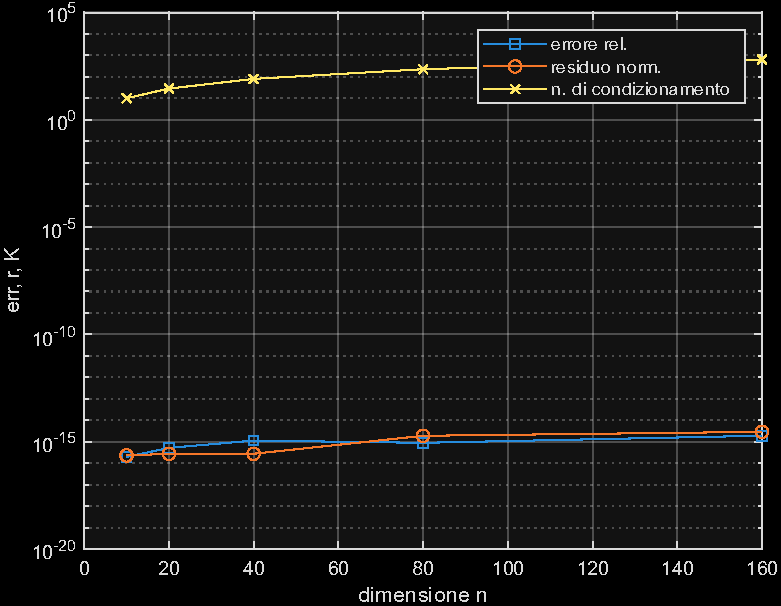
\includegraphics[width=.7\textwidth]{img/metodi-diretti.pdf}
        \caption{Andamento dell'errore relativo, del residuo normalizzato e del numero di condizionamento in funzione di $n$.}
    \end{figure}
\end{enumerate}

\newpage

\subsubsection{Metodi iterativi}

I metodi iterativi stazionari sono considerati in genere nella seguente forma:
\begin{equation*}
    \mathbf{x}^{\left(k+1\right)} = B\mathbf{x}^{\left(k\right)} + \mathbf{f} \hspace{2em} k \ge 0
\end{equation*}
Dove $B$ è detta matrice di iterazione. $B$ e $\mathbf{f}$ identificano il metodo.

\paragraph{Metodo di Jacobi}

Si consideri la matrice diagonale $D$ degli elementi diagonali di $A$. Tale matrice è facilmente invertibile, se gli $a_{ii} \ne 0, i = 1, \dots, n$, in quanto:
\begin{equation*}
    D = \begin{pmatrix}
        a_{11}  & 0     & 0     & \cdots    & 0     \\
        0       & a_{22}& 0     & \cdots    & 0     \\
        \vdots  & 0     & \ddots& \ddots    & \vdots\\
        \vdots  & \vdots& \ddots& \ddots    & 0     \\
        0       & 0     & \cdots& 0         & a_{nn}
    \end{pmatrix}
    \Longrightarrow
    D^{-1} = \begin{rowequmat}{ccccc}
        \dfrac{1}{a_{11}}   & 0                 & 0     & \cdots    & 0     \\ [.3em]
        0                   & \dfrac{1}{a_{22}} & 0     & \cdots    & 0     \\ [.3em]
        \vdots              & 0                 & \ddots& \ddots    & \vdots\\ [.3em]
        \vdots              & \vdots            & \ddots& \ddots    & 0     \\ [.3em]
        0                   & 0                 & \cdots& 0         & \dfrac{1}{a_{nn}}
    \end{rowequmat}
\end{equation*}
E il metodo può essere scritto direttamente in forma matriciale:
\begin{gather*}
    \mathbf{x}^{\left(0\right)} \text{ assegnato} \\
    \mathbf{x}^{\left(k+1\right)} = B_{J}\mathbf{x}^{\left(k\right)} + \mathbf{f}_{J} \\
\end{gather*}
Dove $B_{J} = I - D^{-1} A = D^{-1} \left(D-A\right)$ è la matrice di iterazione di Jacobi e $\mathbf{f}_{J} = D^{-1} \mathbf{b}$

\paragraph{Metodo di Gauss-Seidel}

Questo metodo si differenza dal metodo di Jacobi per il fatto che considera, oltre alla matrice $D$, anche le due matrici $-E$ e $-F$ triangolari superiore e inferiore della matrice $A$, ovvero:
\begin{equation*}
    -E = \begin{bmatrix}
        0 & 0 & 0 & \cdots &  0 \\
        a_{21} & 0 & 0 & \cdots & 0 \\
        \vdots & a_{32} & \ddots & \ddots & \vdots \\
        \vdots & \vdots & \ddots & \ddots & 0 \\
        a_{n1} & a_{n2} & \cdots & a_{nn-1} & 0
    \end{bmatrix}
    \hspace{2em}
    -F = \begin{bmatrix}
        0 & a_{12} & a_{13} & \cdots & a_{1n} \\
        0 & 0 & a_{23} & \cdots & a_{2n} \\
        \vdots & 0 & \ddots & \ddots & \vdots \\
        \vdots & \vdots & \ddots & \ddots & a_{n-1n} \\
        0 & 0 & \cdots & 0 & 0
    \end{bmatrix}
\end{equation*}
Dunque, il seguente algoritmo o le seguenti istruzioni:
\begin{gather*}
    \mathbf{x}^{\left(0\right)} \text{ assegnato} \\
    \mathbf{x}^{\left(k+1\right)} = B_{GS}\mathbf{x}^{\left(k\right)} + \mathbf{f}_{GS} \\
\end{gather*}
Dove $B_{GS} = \left(D-E\right)^{-1}F$ è la matrice d'iterazione di Gauss-Seidel e $\mathbf{f}_{GS} = \left(D-E\right)^{-1}\mathbf{b}$.

\paragraph{Esercizio}

Si considerino la matrice:
\begin{equation*}
    A = \begin{bmatrix}
        9 & -3 & 1 & & & & \\
        -3 & 9 & -3 & 1 & & & \\
        1 & -3 & 9 & -3 & 1 & & \\
        & 1 & -3 & 9 & -3 & 1 & \\
        && 1 & -3 & 9 & -3 & 1 \\
        &&& 1 & -3 & 9 & -3 \\
        &&&& 1 & -3 & 9 
    \end{bmatrix}
\end{equation*}
E il termine noto:
\begin{equation*}
    \mathbf{b} = \begin{bmatrix}
        7 & 4 & 5 & 5 & 5 & 4 & 7 
    \end{bmatrix}^{T}
\end{equation*}
\begin{enumerate}
    \item Costruire la matrice $A$ (utilizzando i comandi Matlab \texttt{diag} e \texttt{ones}) e determinare il numero di elementi non nulli tramite il comando \texttt{nnz}. La matrice $A$ è a dominanza diagonale per righe? È simmetrica e definita positiva?
    
    È stato richiesto di utilizzare i comandi \texttt{diag} e \texttt{ones} per costruire la matrice $A$. Quindi per farlo, si controlla rapidamente la documentazione dei due comandi:
    \begin{lstlisting}[language=bash]
>> help ones
 ones - Create array of all ones
    This MATLAB function returns the scalar 1.

    Syntax
      X = ones
      X = ones(n)
      X = ones(sz1,...,szN)
      X = ones(sz)

      X = ones(___,typename)
      X = ones(___,'like',p)

    Input Arguments
      n - Size of square matrix
        integer value
      sz1,...,szN - Size of each dimension
        two or more integer values
      sz - Output size
        row vector of integer values
      typename - Output class
        'double' (default) | 'single' | 'logical' | 'int8' | 'uint8' | ...
      p - Prototype
        variable

>> help diag
 diag - Create diagonal matrix or get diagonal elements of matrix
    This MATLAB function returns a square diagonal matrix with the elements
    of vector v on the main diagonal.

    Syntax
      D = diag(v)
      D = diag(v,k)

      x = diag(A)
      x = diag(A,k)

    Input Arguments
      v - Diagonal elements
        vector
      A - Input matrix
        matrix
      k - Diagonal number
        integer\end{lstlisting}
    Adesso si osservi la matrice $A$. È possibile notare che la diagonale principale ha tutti i valori uguale a $9$, mentre sopra e sotto la diagonale principale, altre due diagonali con valore pari a $-3$ e allo stesso modo due diagonali con valore uguale a $1$.

    Usando entrambi i comandi, si può giungere al seguente risultato parziale:
    \begin{lstlisting}[language=MATLAB]
>> diag(9*ones(1, n)) + diag(-3*ones(1,n-1), 1) + diag(1*ones(1,n-2), 2)

ans =

        9    -3     1     0     0     0     0
        0     9    -3     1     0     0     0
        0     0     9    -3     1     0     0
        0     0     0     9    -3     1     0
        0     0     0     0     9    -3     1
        0     0     0     0     0     9    -3
        0     0     0     0     0     0     9\end{lstlisting}
    Ed eseguendo con la stessa logica anche sotto la diagonale principale, si ottiene la matrice $A$ richiesta:
    \lstinputlisting[language=MATLAB]{code/risoluzione-di-sistemi-di-equazioni-lineari/metodi-iterativi/J_GS_1.m}

    Il numero di elementi non nulli si calcola con il comando \texttt{nnz}:
\begin{lstlisting}[language=bash]
>> help nnz
 nnz - Number of nonzero matrix elements
    This MATLAB function returns the number of nonzero elements in matrix X.

    Syntax
      N = nnz(X)

    Input Arguments
      X - Input matrix
        matrix

>> nnz(A)

ans =

    29
\end{lstlisting}
    E infine, per confermare che la matrice sia a dominanza diagonale per righe, simmetrica e definita positiva:
    \lstinputlisting[language=MATLAB]{code/risoluzione-di-sistemi-di-equazioni-lineari/metodi-iterativi/J_GS_2.m}


    \item Si calcolino le matrici di iterazione:
    \begin{gather*}
        B_{J} = D^{-1}\left(D - A\right) \\
        B_{GS} = \left(D - E\right)^{-1}F
    \end{gather*}
    Associate rispettivamente ai metodi di Jacobi e Gauss-Seidel e i relativi raggi spettrali. La condizione necessaria e sufficiente per la convergenza del metodo iterativo è soddisfatta in entrambi i casi?

    Le matrici di iterazione dei due metodi si calcolano a partire dalla definizione:
    \lstinputlisting[language=MATLAB]{code/risoluzione-di-sistemi-di-equazioni-lineari/metodi-iterativi/J_GS_3.m}

    Si noti l'istruzione \texttt{D = diag(diag(A))}; il comando interno estrae la diagonale principale di $A$, restituendo un vettore, il quale viene elaborato dal comando più esterno che crea una seconda matrice quadrata identica alla dimensione di $A$ ma con solo la diagonale principale.

    Dal calcolo del raggio spettrale delle matrici si può concludere che in questo caso entrambi i metodi convergono, in quanto l'autovalore massimo risulta in modulo strettamente minore di 1. Si osservi che il raggio spettrale della matrice di iterazione del metodo di Gauss-Seidel è più basso di quello della matrice del metodo di Jacobi.

    \item Scrivere la funzione Matlab che implementi il metodo di Jacobi inversione \emph{matriciale} per il sistema lineare $A\mathbf{x} = \mathbf{b}$. L'intestazione della funzione sarà la seguente:
    \begin{equation*}
        \texttt{[x,k] = jacobi(A,b,x0,toll,nmax).}
    \end{equation*}
    Il processo iterativo si arresta quando:
    \begin{equation*}
        \dfrac{\left|\left|\mathbf{r}^{(k)}\right|\right|}{\left|\left|\mathbf{b}\right|\right|} \leq \texttt{toll}
    \end{equation*}
    (criterio d'arresto del residuo normalizzato).

    \lstinputlisting[language=MATLAB]{code/risoluzione-di-sistemi-di-equazioni-lineari/metodi-iterativi/jacobi.m}

    \item Scrivere una funzione Matlab che implementi il metodo di Gauss-Seidel inversione \emph{matriciale} per il sistema lineare $A\mathbf{x} = \mathbf{b}$. L'intestazione della funzione sarà la seguente:
    \begin{equation*}
        \texttt{[x,k] = gs(A,b,x0,toll,nmax).}
    \end{equation*}

    \lstinputlisting[language=MATLAB]{code/risoluzione-di-sistemi-di-equazioni-lineari/metodi-iterativi/gs.m}

    \item Costruire il termine noto $\mathbf{b}$. Utilizzando le funzioni costruite nei punti 3 e 4, risolvere il sistema $A\mathbf{x} = \mathbf{b}$ ponendo $x^{(0)} = \left[0,0,\dots,0\right]^{T}$, $\texttt{toll} = 10^{-6}$ e $\texttt{nmax} = 1000$. Confrontare il numero di iterazioni necessarie per arrivare a convergenza per i due metodi e commentare i risultati ottenuti.
    
    Il metodo di Gauss-Seidel converge più velocemente alla soluzione esatta in accordo con il corrispondente raggio spettrale che è più basso di quello della matrice del metodo di Jacobi.
    \lstinputlisting[language=MATLAB]{code/risoluzione-di-sistemi-di-equazioni-lineari/metodi-iterativi/J_GS_4.m}
\end{enumerate}


    %%%%%%%%%%%%%%%%%%%%%%%%%%
    % Bibliography and index %
    %%%%%%%%%%%%%%%%%%%%%%%%%%
    \pagestyle{fancy}
\fancyhead{} % clear all header fields
\fancyhead[R]{\nouppercase{\leftmark}}

\bibliography{bibtex}{}
\bibliographystyle{plain}

\newpage

\printindex
\end{document}